\tit{Partial lexicographic preference trees}, or \tit{PLP-trees}, form
an intuitive formalism for compact representation of qualitative 
preferences over combinatorial domains. 
In this chapter, we show that PLP-trees can be 
used to accurately model preferences arising in practical situations, and 
that high-accuracy PLP-trees can be effectively computed. We also propose 
and study a variant of the model based on the concept of a \emph{PLP-forest},
a \emph{collection} of PLP-trees, where the preference order specified by a 
PLP-forest is obtained by aggregating the orders of its constituent PLP-trees. 
The motivation is that learning many PLP-trees, each from a small set of 
examples, often is faster than learning a single tree from a large example
set yet, thanks to aggregation, yields an accurate and robust representation 
of the preference order being modeled. We propose and implement several algorithms 
to learn PLP-trees and PLP-forests. To support experimentation, we use 
datasets that we adapted to the preference learning setting from existing 
classification datasets.
Our results demonstrate the potential of both approaches, with learning 
PLP-forests showing particularly promising behavior.


\section{Introduction}
Learning
preference models, that is, expressions concisely representing a 
preference order has been central to this research. Much of the 
attention was focused on learning utility functions that represent
preference orders quantitatively \cite{furnkranz2011preference}.
Recently, researchers proposed several \emph{qualitative} models of preference 
orders arguing that they are more directly aligned with conventions humans 
use when expressing their preferences. They include \tit{conditional
preference networks} (CP-nets)
\cite{boutilier2004cp}, and models ordering outcomes lexicographically 
such as lexicographic strategies \cite{schmitt2006complexity}, conditional 
lexicographic preference trees \cite{brauning2012learning}, lexicographic preference 
trees (LP-trees) \cite{booth:learningLP}, partial lexicographic preference
trees (PLP-trees)
\cite{conf/aaai15/LiuT}, and preference trees\cite{fraser1994ordinal,%
liu2015reasoning}. As with quantitative models, learning qualitative
models is important. Indeed, eliciting them directly from users is often 
impractical. However, while learning CP-nets has received a fair amount 
of attention \cite{lang2009complexity,dimopoulos2009ceteris,
koriche2010learning,guerin2013learning}, study of learning lexicographic 
models is still in the early stages. The results obtained so far concern mostly 
learning LP-trees \cite{booth:learningLP} and 
conditional lexicographic preference trees \cite{brauning2012learning}. 
Other models received less attention. In particular, no algorithms for
learning PLP-trees have yet been proposed even though
PLP-trees retain the simplicity of LP-trees but also offer flexibility
that makes them less sensitive to overfitting. 

In this chapter, we address the problem of practicality of PLP-trees as 
a preference representation formalism. To this end, we introduce several 
best-agreement and approximate algorithms to learn PLP-trees of the four classes:
UIUP, UICP, CIUP, and CICP (as discussed in \chref{learningPLPT}).
We show experimentally that they are effective on various domains
and datasets and generate trees that accurately approximate the preference 
order being modeled. To support our experiments, following Br{\"a}uning 
and Eyke \cite{brauning2012learning}, we generated a library of datasets 
of preference examples deriving them from datasets of examples developed 
by the machine learning community to support research on the classification 
problem.

PLP-trees are in some aspects similar to decision trees. 
When learning a decision tree, a problem that may arise is that of 
overfitting. To reduce its effect, Breiman \cite{breiman2001random} 
proposed learning a \tit{random forest}, that is, a set of uncorrelated 
decision trees learned from randomly selected sets of examples. The 
random forest learning algorithm \cite{breiman2001random} has two key 
steps. First, it generates several decision trees, randomizing the attributes
used in their construction. Then, to classify an instance, the algorithm 
\tit{aggregates} the predictions made by individual trees in the forest 
by the majority rule. 

We adapted both the notion of a decision forest and 
the idea to aggregate their elements to the 
setting of PLP-trees. A \emph{PLP-forest} is a collection of PLP-trees. 
PLP-forests consisting exclusively of UIUP, UICP, CIUP or CICP trees are
called UIUP, UICP, CIUP or CICP PLP-forests, respectively.
PLP-trees in a PLP-forest are learned using randomly selected \tit{small} 
fragments of a training set. To predict if one outcome is preferred over 
another, we apply the \tit{pairwise majority rule} (PMR), a simple and 
effective voting rule studied in social choice. We adjust algorithms 
learning PLP-trees to the setting of PLP-forests and study their 
effectiveness both in terms of time and accuracy.

The key findings supported by our results are: (1) PLP-trees and PLP-forests 
are expressive preference models. Experiments with the datasets we constructed 
from commonly used machine learning classification domains showed that the
accuracy of learned models typically exceeded 85\%, often exceeded 90\%, and 
in some cases was as high as 95\%. (2) PLP-forests aggregated by PRM provide 
in general higher accuracy than PLP-trees. (3) PLP-trees and PLP-forests 
learned by a greedy approximation method have accuracy comparable to 
\emph{best-agreement} PLP-trees and PLP-forests learned by maximizing the
number of correctly handled examples in the training set. Moreover, because of 
overfitting arising in ``best-agreement'' trees and forests, in some cases, heuristic 
approaches offer an even better accuracy. (4) Approximation learning methods 
are fast and can work with large datasets; methods based on learning 
best-agreement trees can also be effective in practice, especially when we 
learn PLP-forests, where we bound the number of examples each tree in the
forest is learned from.

This chapter is organized as follows. In \secref{trees}, we begin with reviewing
PLP-trees and their classification, extending them to domains with arbitrary
multi-valued (that is, not necessarily binary) attributes. We also recall 
the complexity of the problem to learn PLP-trees \cite{conf/aaai15/LiuT}. 
We also discuss the preference learning library that we
use in our experiments. Next, we discuss algorithms to
learn PLP-trees. We consider two types of algorithms --- finding best-agreement
PLP-trees and finding PLP-trees based on the greedy heuristics. 
We then present
and discuss empirical results on the performance of our PLP-tree learning 
algorithms. In \secref{forests}, we introduce PLP-forests and specify the
pairwise majority rule to aggregate trees in a PLP-forest. This is followed by 
an analysis of experimental results using the same datasets as before. We 
conclude the chapter with a brief summary and a look into possible 
directions for future work.


\section{Partial Lexicographic Preference Trees}
\label{sec:trees}
We study the four classes of PLP-trees: UIUP, UICP, CIUP, and CICP.
Among UICP trees, of practical interest are those where the number of
parents are bounded by some fixed integer $k$ independent of $p$, and 
the CPTs are complete. We call this type of trees UICP-$k$ PLP-trees.
In this case, the sizes of the CPTs and, consequently, the sizes of the trees 
are polynomial in the number of attributes.
In practice, when deciding a preference order at an attribute,
humans rarely condition them on more than two attributes of higher importance.
Consider the domain of cars over three binary attributes:
\tit{Capacity}, \tit{Price} and \tit{Safety},
with values \tit{high} ($1_1$) and \tit{low} ($0_1$),
\tit{high} ($1_2$) and \tit{low} ($0_2$), and
\tit{high} ($1_3$) and \tit{low} ($0_3$), respectively.
An example of UICP-1 PLP-trees over cars is shown in \figref{UICP1_PLPT_compact}.

\begin{figure}[!ht]
	\centering
	\begin{tikzpicture}[->,>=stealth',
	  level/.style={sibling distance=2cm/#1, level distance=40pt}]
	  \node [main node] (1){$X_1$}
	    child {node [main node] (2) {$X_2$}
	      child {node [main node] (3) {$X_3$} {}
	          child {node [rectangle,draw] (4) at (2,4.2) {$1_1>0_1$} edge from parent[draw=none]}
	          child {node [rectangle split, rectangle split parts=2,draw] (5) at (1.75,2.8)
	            {$1_1:1_2>0_2$ \nodepart{second} $0_1:0_2>1_2$} edge from parent[draw=none]}
	          child {node [rectangle,draw] (6) at (0.7,1.4) {$1_3>0_3$} edge from parent[draw=none]}
	      }
	    };
	\end{tikzpicture}
	\caption{UICP-1 PLP-tree \label{fig:UICP1_PLPT_compact}}
\end{figure}

We now discuss the complexity of the problem to learn
PLP-trees. The problem assumes that we are given a collection of examples,
that is, expressions $(\alpha,\beta,\succ)$ and $(\alpha,\beta,\approx)$,
where $\alpha$ and $\beta$ are outcomes. Examples of the first type are
\emph{strict} examples and of the second type \emph{equivalence} examples.
A PLP-tree $T$ satisfies a strict example $(\alpha,\beta,\succ)$ if $\alpha
\succ_T \beta$. Similarly, $T$ satisfies an equivalence example $(\alpha,
\beta,\approx)$ if $\alpha\approx_T\beta$. The objective of the problem
is to compute a PLP-tree (of a specified type) that satisfies the maximum
number of examples from the input set. We refer to this problem as
\tsc{MaxLearn}.

The \tsc{MaxLearn} problem is NP-hard for each of the four classes of
PLP-trees we discussed (when applicable, assuming that we learn collapsed
representations). This is an easy consequence of the fact that the
corresponding decision versions of the problem (asking for the existence
of a PLP-tree of a given type satisfying at least $k$ examples from the
input set, where $k$ is another input parameter) are NP-complete
\cite{conf/aaai15/LiuT}.

\subsection{Preference Learning Library}
\label{sec:library}
We now describe the datasets we used in our study of learning algorithms
we present later. These datasets were generated from publicly available 
classification datasets developed by the machine learning community. 
%To prevent the exact method from handling too large search spaces,
When constructing the datasets, we limited the number of attributes 
in outcomes to ten and the sizes of attribute domains to four. 

Classification datasets associate with each outcome $\alpha$ a label
$l(\alpha)$. If there is a total (pre)order relation on the labels, say
$\succeq$, we can use this relation to produce preference examples out of
classification examples. Namely, for each pair of outcomes $\alpha$ and $\beta$
from the classification dataset, if $l(\alpha) \succ l(\beta)$, we take 
$(\alpha,\beta,\succ)$ as a strict example, and if $l(\alpha)= l(\beta)$, 
we take $(\alpha,\beta,\approx)$ as an equivalence example.\footnote{Clearly, 
our preference datasets do not contain incomparability examples. This is not 
a limitation in our work as the preference models we learn represent total 
preorders.} Throughout the chapter, we write $p$ for the number of attributes
in a dataset, $\cX$ for the set of outcomes, $\cE$ for the set of examples, 
and $\cE^{\succ}$ and $\cE^{\approx}$ for the sets of strict and equivalence
examples, respectively.

%The idea is to associate an order with the labels used in
%a classification dataset.
%For each dataset, we impose \tit{total order} on the labels
%so that we derive a \tit{total preorder}, that is total,
%reflexive and transitive, over the instances, or outcomes.
%From this total preorder, we produce pairwise preferences
%in $\cE^\succ$ and $\cE^\approx$ so that
%$(\alpha,\beta) \in \cE^\succ$ $\itiff$ the label of outcome
%$\alpha$ precedes that of $\beta$ in the total preorder,
%and $(\alpha,\beta) \in \cE^\approx$ $\itiff$
%the labels of outcomes $\alpha$ and $\beta$ are the same.

\begin{table}
        \centering
        \small
        \caption{Classification datasets in UCI Machine Learning Repository 
								 used to generate preference datasets}
        \begin{tabular}{ |c||c| }
                \hline
                Preference Datasets    & Original Datasets in UCI MLR \\
                \hline \hline
                BreastCancerWisconsin  & Breast Cancer Wisconsin \\
                \hline
                CarEvaluation          & Car Evaluation \\
                \hline
                CreditApproval         & Credit Approval \\
                \hline
                GermanCredit           & Statlog (German Credit Data) \\
                \hline
                Ionosphere             & Ionosphere \\
                \hline
                MammographicMass       & Mammographic Mass \\
                \hline
                Mushroom               & Mushroom \\
                \hline
                Nursery                & Nursery \\
                \hline
                SPECTHeart             & SPECT Heart \\
                \hline
                TicTacToe              & Tic-Tac-Toe Endgame \\
                \hline
                Vehicle                & Statlog (Vehicle Silhouettes) \\
                \hline
                Wine                   & Wine \\
                \hline
        \end{tabular}
        \label{tbl:class}
\end{table}


At present, our preference library consists of twelve datasets obtained 
from the classification datasets listed in \tblref{class}. 
In ten of them %(e.g., CarEvalation)
there is a natural order on the labels. 
%for which we apply a natural order over their labels.
For the other two of them namely, Vehicle and Wine, 
there is no domain-specific natural order on the labels. In these two cases, 
to generate examples we fixed a preference order on the labels arbitrarily 
(see below).
We discuss three preference datasets (CarEvaluation, Vehicle and Wine) 
in detail and provide a summary description
of the remaining ones in \tblref{description}, where
we use $|\cdot|$ to denote the size of a set.

%\smallskip \noindent \textbf{BreastCancerWisconsin \ }
%The BreastCancerWisconsin dataset has 270 outcomes over 9 attributes.
%To generate equivalent and strict examples for the dataset,
%we assume that outcomes labeled by ``benign" are better than
%those by ``malignant."
%For equivalent examples, we have that outcomes labeled by ``benign" are equivalent
%to one another, so are those labeled by ``malignant."

\smallskip \noindent \textbf{CarEvaluation \ }
The CarEvaluation dataset has 1728 outcomes over 6 attributes.
To generate equivalent and strict examples for the dataset,
we assume that outcomes labeled by ``vgood" are better than
those by ``good," which are better than those
by ``acc," which are preferred to those by ``unacc."

%\smallskip \noindent \textbf{CreditApproval \ }
%The CreditApproval dataset has 520 outcomes over 10 attributes.
%To generate equivalent and strict examples for the dataset,
%we assume that outcomes labeled by ``+" (positive) are better than
%those by ``-" (negative).
%
%\smallskip \noindent \textbf{GermanCredit \ }
%The GermanCredit dataset has 914 outcomes over 10 attributes.
%To generate equivalent and strict examples for the dataset,
%we assume that outcomes labeled by ``1" (good) are better than
%those by ``2" (bad).
%
%\smallskip \noindent \textbf{Ionosphere \ }
%The Ionosphere dataset has 118 outcomes over 10 attributes.
%To generate equivalent and strict examples for the dataset,
%we assume that outcomes labeled by ``g" (good) are better than
%those by ``b" (bad).
%
%\smallskip \noindent \textbf{MammographicMass \ }
%The MammographicMass dataset has 118 outcomes over 10 attributes.
%To generate equivalent and strict examples for the dataset,
%we assume that outcomes labeled by ``0" (benigh) are better than
%those by ``1" (malignant).
%
%\smallskip \noindent \textbf{Mushroom \ }
%The Mushroom dataset has 184 outcomes over 10 attributes.
%To generate equivalent and strict examples for the dataset,
%we assume that outcomes labeled by ``e" (edible) are better than
%those by ``p" (poisonous).
%
%\smallskip \noindent \textbf{Nursery \ }
%The Nursery dataset has 184 outcomes over 10 attributes.
%To generate equivalent and strict examples for the dataset,
%we assume that outcomes labeled by ``spec\_prior" are better than
%those by ``priority," which are better than those
%by ``very\_recom," which are preferred to those by ``recommend,"
%which again are better than those by ``not\_recom."
%
%\smallskip \noindent \textbf{SPECTHeart \ }
%The SPECTHeart dataset has 115 outcomes over 10 attributes.
%To generate equivalent and strict examples for the dataset,
%we assume that outcomes labeled by ``0" (positive) are better than
%those by ``1" (negative).
%
%\smallskip \noindent \textbf{TicTacToe \ }
%The TicTacToe dataset has 958 outcomes over 9 attributes.
%To generate equivalent and strict examples for the dataset,
%we assume that outcomes labeled by ``positive" are better than
%those by ``negative".

\smallskip \noindent \textbf{Vehicle \ }
The Vehicle dataset has 455 outcomes over 10 attributes.
To generate equivalent and strict examples for the dataset,
we assume that outcomes labeled by ``bus" are better than
those by ``opel," which are better than those
by ``saab," which are preferred to those by ``van."

\smallskip \noindent \textbf{Wine \ }
The Wine dataset has 177 outcomes over 10 attributes.
To generate equivalent and strict examples for the dataset,
we assume that outcomes labeled by ``1" are better than
those by ``2," which are better than those
by ``3."


\begin{table}
	\centering
	\small
	\caption{Description of datasets in the library}
	\begin{tabular}{ |c||c|c|c|c| } 
		\hline
		Dataset          & $p$  & $|\cX|$ & $|\cE^\succ|$ & $|\cE^\approx|$ \\
		\hline \hline
		BreastCancerWisconsin              & 9    & 270 & 9,009 & 27,306 \\ \hline
		CarEvaluation               & 6    & 1,728 & 682,721 & 809,407\\ \hline
		CreditApproval               & 10   & 520 & 66,079 & 68,861 \\ \hline
		GermanCredit               & 10   & 914 & 172,368 & 244,873 \\ \hline
		Ionosphere               & 10   & 118 & 3,472 & 3,431 \\	\hline
		MammographicMass               & 5    & 62 & 792 & 1,099 \\	\hline
		Mushroom               & 10   & 184 & 8,448 & 8,388 \\	\hline
		Nursery               & 8    & 1,266 & 548,064 & 252,681 \\	\hline
		SPECTHeart               & 10   & 115 & 3,196 & 3,359 \\	\hline
		TicTacToe              & 9    & 958 & 207,832 & 250,571 \\ \hline
		Vehicle               & 10   & 455 & 76,713 & 26,572 \\ \hline
		Wine               & 10   & 177 & 10,322 & 5,254 \\
		\hline
	\end{tabular}
	\label{tbl:description}
\end{table}


\subsection{Algorithms}
\label{sec:algs}
We propose and evaluate both best-agreement and 
greedy algorithms for the \tsc{MaxLearn} problem. 
For these algorithms and experiments, we focus on solving the
\tsc{MaxLearn} problem where the given the set of examples
contains only strict examples.
The learning algorithms are essentially to learn PLP-trees that
approximate the original total preorders of at most five
equivalent clusters of outcomes.
A small PLP-tree with three or more nodes will already specify
a preorder of more clusters.
Our algorithms typically learn bigger trees.
Thus, learning these tie-breaking trees provides finer-grained
approximations of the original orderings and better
understanding of the distribution of the outcomes according
to the agents' preferences.

To find the best-agreement model, that is, to
compute a PLP-tree (of a specified type) that maximizes the number of 
satisfied examples, we used answer-set programming (ASP)
\cite{marek1999stable,niemela1999logic} and its \emph{gringo/clasp}
grounder-solver tool \cite{gebser2011potassco}.
This approach consists of two logical programming modules: 
the data module
describing the dataset (i.e., attributes, domains, outcomes and examples),
and the rule module applying an optimization statement to search for
a PLP-tree that correctly decides as many examples as possible.
Given an instance of the \tsc{MaxLearn} problem expressed as the two modules,
the ASP tool \emph{gringo/clasp} computes an answer set encoding the PLP-tree
that is a solution to the input instance.

Our method to solve the \tsc{MaxLearn} problem approximately, that is, to 
compute a PLP-tree that satisfies many (but perhaps not the maximum
possible) number of examples is based on a greedy approach.

\algref{recur_learn} provides a detailed description of the method. When
the Boolean parameter $\Delta$ is set to \tbf{true}, the algorithm learns $\UI$ 
trees, otherwise, it learns $\CI$ trees with conditional importance of attributes. 
The algorithm starts with a non-empty container (e.g., a stack or a queue) $C$
of one item $(\cE^\succ,\cA,n,\Delta)$ and an unlabeled node $T$ set to $n$.
We now describe the remainder of \algref{recur_learn} for each value of
$\Delta$ (learning UI and CI trees, respectively).

\smallskip \noindent \tbf{UI \ }
The algorithm pops an item $(\cE^\succ,\cA,n,\Delta)$ from $C$, and
picks the root attribute $X_l$ and
$CPT(X_l)$ that correctly handles the most examples in $\cE$.
Next, it updates the set $\cA$ of available attributes and the
set $\cE$ of remaining examples to be decided, and creates 
the next node $n'$.  Then, the algorithm creates and pushes the item
$(\cE^\succ,\cA,n',\Delta)$ onto $C$.
The algorithm repeats until all strict
examples in $\cE^\succ$ are decided, either correctly or not.
For UIUP trees, the $CPT(X_l)$ has only a single local preference.
For UICP-1 trees, the table could contain only one local preference
as in the UIUP case, or it could be a $CPT(X_l)$ of preferences on
$D_l$ dependent on one parent attribute (cf. \figref{UICP_PLPT_compact}).

\smallskip \noindent \tbf{CI \ }
As in the case of UI trees, the algorithm pops an item from $C$,
and picks $(X_l,CPT(X_l))$
for the root, where $CPT(X_l)$ contains only one local preference.
Having updated $\cA$ and $\cE$, for each value of $X_l$,
the algorithm constructs a node and partitions $\cE$.
Next, when the algorithm pushes all items $(\cE^\succ_i,\cA,n_i,\Delta)$
onto to container $C$, the choice of $C$ could make a difference on
the CIUP tree to be learned.
This is because the local preference learned for an attribute is fixed
for that attribute which could appear elsewhere in the tree.
To this end, we implemented $C$ using stack and queue in our
experiments to have the learning algorithm for CIUP trees work either
in a breadth-first or a depth-first manner.
We hereby denote by CIUPB (CIUPD) the class of CIUP trees
learned by the breadth-first (depth-first, respectively) implementation
of the greedy algorithm.
However, for the most general type of CI trees, the CICP PLP-trees, 
the choice does not influence the quality of the learned models.

\begin{algorithm}[ht]
\KwIn{$C$: a container of items $(\cE^\succ,\cA,n,\Delta)$, where $\cE^\succ$ is the set of
			strict example to be decided, $\cA$ the set of available attributes,
			$n$ an unlabeled node to consider next, 
			and $\Delta$ a Boolean value indicating the type
			of PLP-trees (UI or CI) to be learned, and
			$T=n$: an unlabeled node for which a PLP-tree is to be learned.}
\KwOut{A PLP-tree $T$ over $\cA$.}
	$(\cE^\succ,\cA,n,\Delta) \leftarrow$ Pop an item from $C$\;
	\uIf{$\cE^\succ = \emptyset$}{
		Label $n$ as a leaf\;
		\If{$C$ is empty}{
			\Return\;
		}
	}
	\Else{
		$(X_l,CPT(X_l)) \leftarrow$ Pick $X_l \in \cA$ and $CPT(X_l)$ that correctly
			decides the maximum number of examples in $\cE^\succ$\;
		Label $n$ with tuple $(X_l,CPT(X_l))$\;
		$\cE^\succ \leftarrow \cE^\succ \backslash \{e \in \cE^\succ: \alpha_e(X_l)\not=\beta_e(X_l)\}$\;
		$\cA \leftarrow \cA \backslash \{X_l\}$\;
		\uIf{$\Delta = \tbf{true}$}{
			Create an edge $u$ and an unlabeled node $n'$ such that $u=\langle n,n'\rangle$\;
			Push item $(\cE^\succ,\cA,n',\Delta)$ onto $C$\;
		}
		\Else{
			\For{$i \leftarrow 1$ to $|D_l|$}{
				Create an edge $u_i$ and an unlabeled node $n_i$ such that $u_i=\langle n,n_i\rangle$\;
				$\cE^\succ_i \leftarrow \{e\in \cE^\succ: \alpha_e(X_l)=\beta_e(X_l)=x_{l,i}\}$\;
				Push item $(\cE^\succ_i,\cA,n_i,\Delta)$ onto $C$\;
			}
		}
	}
	$\mathit{greedy}(C,T)$\;

\caption{The \tit{greedy} algorithm that learns a PLP-tree \label{alg:recur_learn}}
\end{algorithm}

Our greedy method is similar to the greedy method proposed by Schmitt and 
Martegnon \cite{schmitt2006complexity} to learn the so called $\UI$$\FP$ 
trees.\footnote{They are $\UI$$\UP$ trees in which the order on the
values of the domain of every attribute is fixed \emph{a priori} and must
be used in the tree.} Schmitt and Martegnon provided a worst-case performance 
bound for their method. Given a set $\cE$ of preference examples, let 
$\opt(\cE)$ be the minimum number of examples falsified by a $\UI$$\FP$ 
tree, and $\Greedy(\cE)$ be the number of examples falsified by the 
$\UI$$\FP$ tree computed by the greedy approach. Schmitt and Martegnon 
proved that for every set $\cE$ of preference examples over $p$-attribute 
outcomes,
\[
\Greedy(\cE) \leq p \cdot \opt(\cE). 
\]
%This result can be extended to the four classes of PLP-trees we consider
%in this paper. Let $Greedy(\cE,T)$ denote the number of examples in $\cE$
%falsified by our greedy algorithm set to learn a tree of type $T$ (where
%$T$ is one of $\UI$$\UP$, $\UI$$\CP$, etc.).

%\begin{thm}
%For every set of preference examples over $p$-attribute outcomes,
%and for type $T$ of PLP-trees ($T$ is one of $\UI$$\UP$, $\UI$$\CP$, etc.),
%\[
%\Greedy(\cE,T) \leq p \cdot \opt(\cE).
%\] 
%\end{thm}
%\begin{prf}
%	We prove the theorem for the most general case for CICP PLP-trees.
%	We prove by induction.
%	If $p=1$, the argument clearly holds.
%	Now we look at when $p>1$.
%	We denote by $\incorrect(X_j,\cE)$ the number of examples in $\cE$
%	falsified having picked $X_j$ at the root with the best preference.
%	Then, we have $\incorrect(X_j,\cE) \leq \opt_\cA(\cE)$.
%	Having picked $X_j$ in the first step, the greedy algorithm
%	will update $\cA'=\cA \backslash \{X_j\}$ and
%	$\cE'=\cE \backslash \{(\alpha,\beta):\alpha(X_j) \not= \beta(X_j)\}$.
%	Then, $\cE'$ is partitioned to $\{\cE_1',\ldots,\cE_{|D_j|}'\}$.
%	Hence, we have 
%	\begin{center}
%		\[\opt_\cA(\cE) \geq \sum_{1 \leq i \leq |D_j|} \opt_\cA(\cE_i')
%			\geq \sum_{1 \leq i \leq |D_j|} \opt_{\cA'}(\cE_i')\].
%	\end{center}
%	Let $T_i'$ be the CICP tree learned by our greedy algorithm using
%	$\cA'$ and $\cE'$.  By the induction hypothesis, we have
%	\begin{center}
%		\[\incorrect(T_i',\cE_i') \leq (p-1) \cdot \opt_{\cA'}(\cE_i').\]
%	\end{center}
%	Thus, we have the following.
%	\begin{equation*}
%		\begin{split}
%			\incorrect(T,\cE) &= \incorrect(X_j,\cE) + \\
%												&\sum_{1 \leq i \leq |D_j|} \incorrect(T_i',\cE_i') \\
%												&\leq \opt_\cA(\cE) + \\
%												&\sum_{1 \leq i \leq |D_j|}\Big( (p-1) \cdot \opt_{\cA'}(\cE_i') \Big) \\
%												&= \opt_\cA(\cE) + \\
%												&(p-1) \cdot \sum_{1 \leq i \leq |D_j|}\opt_{\cA'}(\cE_i') \\
%												&\leq \opt_\cA(\cE) + (p-1) \cdot \opt_\cA(\cE) \\
%												&= p \cdot \opt_\cA(\cE).
%		\end{split}
%	\end{equation*}
%\end{prf}

This result does not give a tight bound on the performance of the greedy 
method. Schmitt and Martegnon \cite{schmitt2006complexity} proved that no
polynomial-time algorithm learning $\UI$$\UP$ trees that would be accurate 
to within a constant factor $c$ is possible unless P=NP. We conjecture that
the same holds for more general classes of trees, although it may be that
$p$ in the upper bound can be replaced by a slower growing function of $p$.   
We leave these questions for future work and focus here on experimental
evaluation of the accuracy of our learning algorithms.


\subsection{Experiments}
\label{sec:exp_trees}
First, we consider learning UIUP PLP-trees using the 
best-agreement and greedy methods. The goal is to compare the accuracy of
both methods. This is important as the best-agreement method, because of 
its complexity, can only be used on relatively small example sets. 

For a dataset $D$ (where $D$ is one of the twelve datasets we studied),
we fix the size of the training set to $t$, where $1\leq t\leq 250$. 
Then, we randomly pick $\TR_D \subset \strictEx$, where $|\TR_D|=t$, 
as the set of 
\tit{training} examples, and $\TE_D = \strictEx \setminus \TR_D$ as the set 
of \tit{testing} examples. Then, from $\TR_D$, we train a UIUP PLP-tree 
$T_\BA$ using the best-agreement method (that is, $T_\BA$ decides the maximum
possible number of examples in $\TR_D$), and a UIUP PLP-tree $T_G$ using 
our greedy heuristics. Finally, we test the models $T_\BA$ and $T_G$, on the testing examples in 
$\TE_D$ and compute the \emph{accuracy} of each method, the percentage of 
strict examples in $\TE_D$ decided correctly by the corresponding tree. 
For each $t$, $1\leq t\leq 250$, we repeat this process $20$ times and 
compute the average accuracies. We do this for all 12 datasets. 
\figref{trees1} shows the \emph{learning curves} (the accuracies as the function of the
size of the training set) for the the best-agreement method (BA-UIUP)
and the greedy algorithm (G-UIUP)
for the datasets CarEvaluation, Ionosphere, Mushroom and Wine. 
We show the accuracies for the two methods on all datasets when 
$t=|\TR_D|=250$ in \tblref{trees1}.

This experiment shows that, when the number of training examples 
is small, the greedy approach achieves accuracy comparable with that of
the best-agreement method. The results summarized in \tblref{trees1} show 
that (1) the greedy algorithm already achieves accuracy exceeding 85\%
on six datasets (notably, accuracy of $95.5\%$ on Wine); and (2) the 
greedy algorithm performs very close to the best-agreement method, with the
difference within 2 percentage points on \emph{all but two datasets}, Ionosphere and 
Mushroom. Examining the learning curves in \figref{trees1}, we observe 
that, on all datasets but Ionosphere and Mushroom,
the greedy algorithm works well compared with the best-agreement method
across the range of the training set sizes. 
The learning curves for the two 
datasets on which the greedy method lags behind the best-agreement one are 
shown in \figref{I1} and \figref{Mush1}.

%What we have learned from \figref{trees1}:
%\begin{enumerate}
%	\item For the exact learning method using ASP (X-UIUP),
%				learned UIUP trees achieve over 70\% of accuracy across all datasets using small 
%				samples of 250 examples:
%				70\%-80\%: 3 datasets, 80\%-90\%: 5 datasets, and 90\%-100\%: 4 datasets.
%	\item For the greedy heuristic method (G-UIUP),
%				t learned UIUP trees achieve also over 70\% of accuracy across all datasets using small
%				samples of 250 examples:
%				70\%-80\%: 5 datasets, 80\%-90\%: 4 datasets, and 90\%-100\%: 3 datasets.
%	\item For the exact search method used in \tit{fitctree}, 
%				a class implemented in the
%				MATLAB Statistics and Machine Learning Toolbox\cite{Matlab}
%				for classification decision tree (DT),
%				learned decision trees achieve over 70\% of accuracy across all datasets using small 
%				samples of 250 examples:
%				70\%-80\%: 2 datasets, 80\%-90\%: 3 datasets, and 90\%-100\%: 7 datasets.
%	\item Comparing X-UIUP and DT, we observe that 
%				X-UIUP performs comparably well with DT, except on two datasets:
%				CarEvaluation and Mushroom, where DT outperforms X-UIUP with big margins.
%				Comparing M-UIUP and DT, we observe similar results.
%				This comparison shows UIUP trees, the simplest PLP-trees, 
%				are mostly as expressive as decision trees
%				in terms of accuracy, when training samples are of
%				small sizes.
%	\item Comparing X-UIUP and G-UIUP, we see that mostly the greedy heuristic is close to
%				the exact algorithm, except for 2 datasets: Ionosphere and Mushroom.
%				This indicates the greedy method works well.
%\end{enumerate}

\begin{table}
  \centering
  \small
  \caption{Accuracy (percentage of correctly handled testing examples)
					 for UIUP PLP-trees learned using the best-agreement and
					 the greedy methods on the learning 
					 data (250 of $\cE^\succ$)}
  \begin{tabular}{ |c||c|c| }
    \hline
    Dataset          & BA-UIUP & G-UIUP \\
    \hline \hline                               
    BreastCancerWisconsin              & 88.4   & 88.2     \\ \hline
    CarEvaluation               & 84.8   & 83.6     \\ \hline
    CreditApproval               & 91.1   & 89.3     \\ \hline
    GermanCredit               & 72.2   & 72.2     \\ \hline
    Ionosphere               & 87.0   & 79.6     \\ \hline
    MammographicMass               & 87.5   & 86.8     \\ \hline
    Mushroom               & 84.8   & 70.3     \\ \hline
    Nursery               & 91.8   & 91.7     \\ \hline
    SPECTHeart               & 93.2   & 92.6     \\ \hline
    TicTacToe              & 72.1   & 71.9     \\ \hline
    Vehicle               & 76.8   & 76.6     \\ \hline
    Wine               & 96.0   & 95.5     \\ \hline
    %WAvg             & 84.2   & 83.6     \\ \hline
  \end{tabular}
  \label{tbl:trees1}
\end{table}

%\begin{figure}[ht]
%	\centering
%
%  \begin{subfigure}[b]{0.23\textwidth}
%		\centering
%  	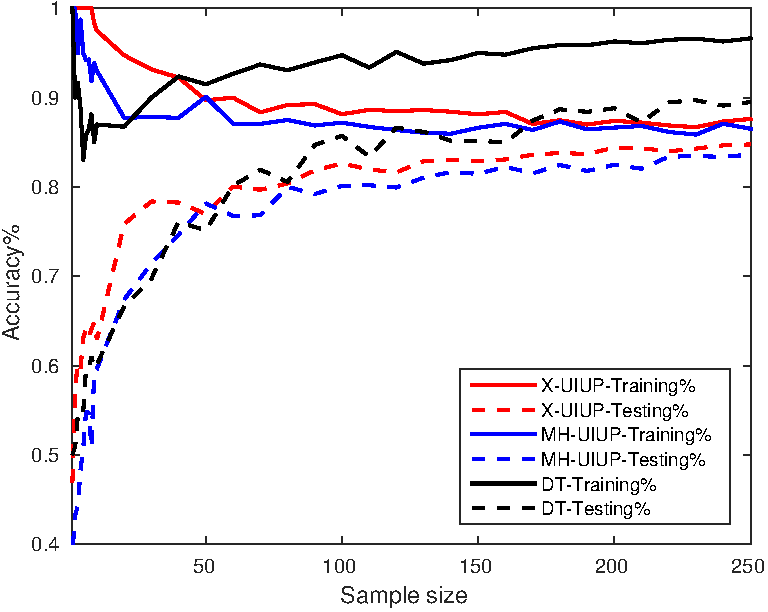
\includegraphics[width=\textwidth]{figs/PLPTF/Trees/CarEvaluation_Trees_X_MH.pdf}
%  	\caption{CarEvaluation}
%		\label{fig:Car1}
%	\end{subfigure}
%  \begin{subfigure}[b]{0.23\textwidth}
%		\centering
%  	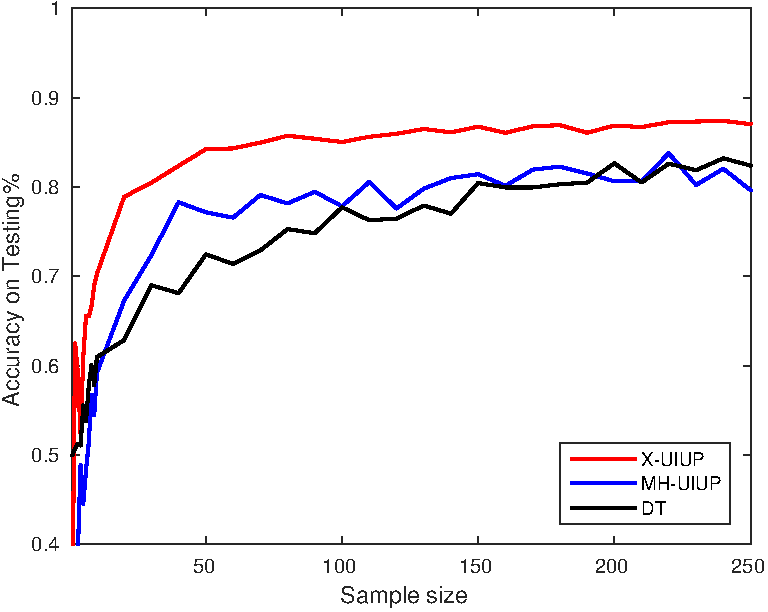
\includegraphics[width=\textwidth]{figs/PLPTF/Trees/IonosphereDownsampledFurther_Trees_X_MH.pdf}
%  	\caption{Ionosphere}
%		\label{fig:I1}
%	\end{subfigure} 
%	\\
%  \begin{subfigure}[b]{0.23\textwidth}
%		\centering
%  	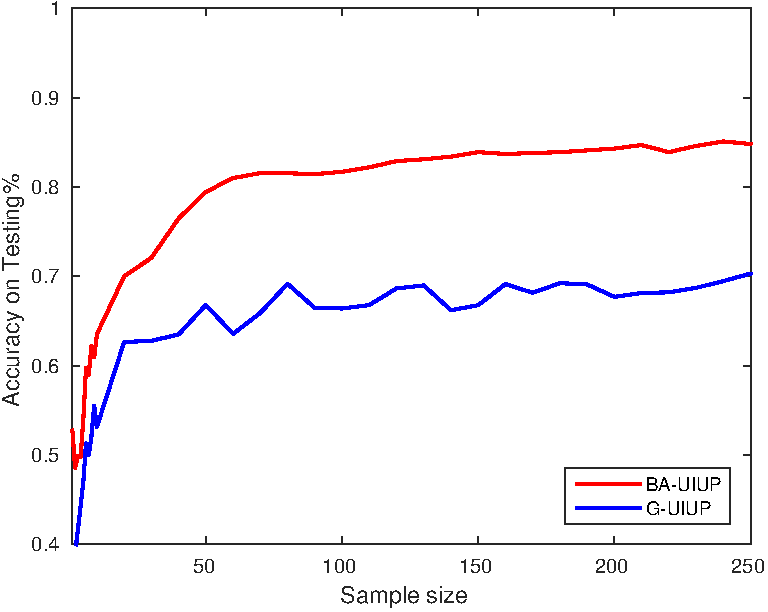
\includegraphics[width=\textwidth]{figs/PLPTF/Trees/MushroomDownsampled_Trees_X_MH.pdf}
%  	\caption{Mushroom}
%		\label{fig:Mush1}
%	\end{subfigure}
%  \begin{subfigure}[b]{0.23\textwidth}
%		\centering
%  	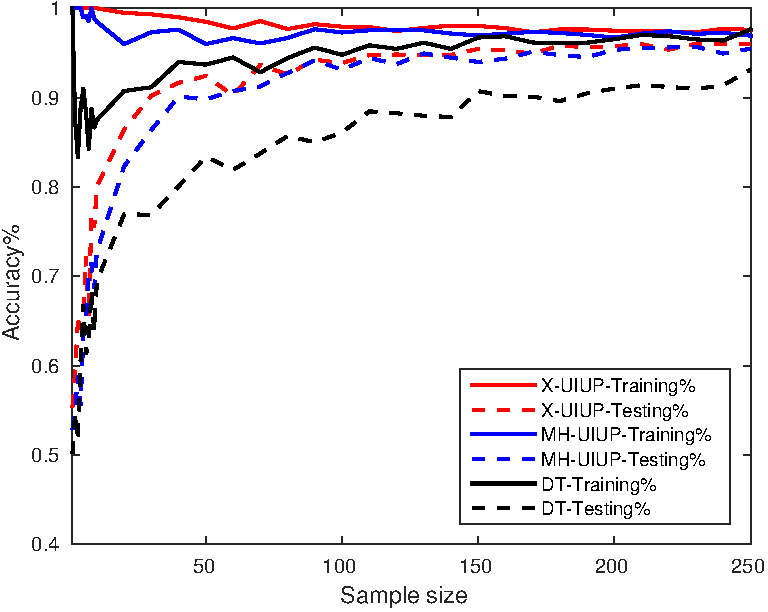
\includegraphics[width=\textwidth]{figs/PLPTF/Trees/WineDownsampled_Trees_X_MH.pdf}
%  	\caption{Wine}
%		\label{fig:W1}
%	\end{subfigure}
%
%  \caption{Learning UIUP PLP-trees}
%  \label{fig:trees1}
%\end{figure}

\begin{figure}[ht]
	\centering

  \begin{subfigure}[b]{0.3\textwidth}
		\centering
		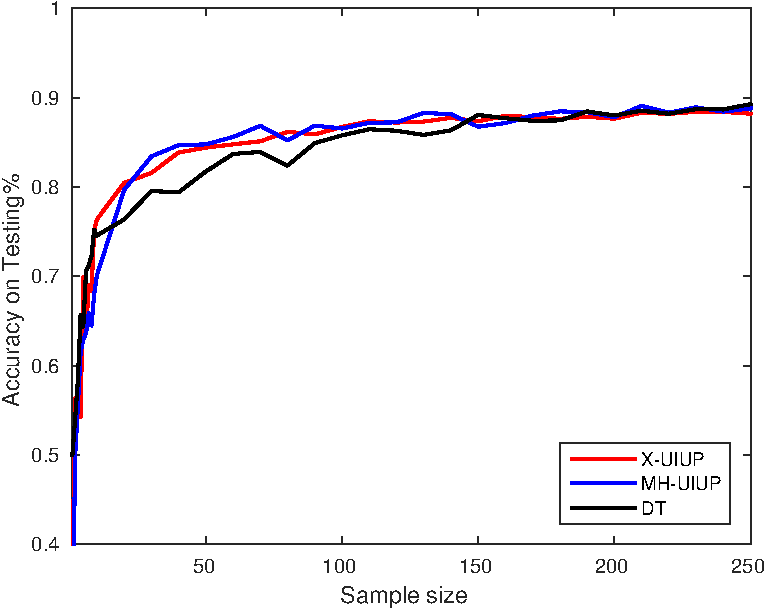
\includegraphics[width=\textwidth]{figs/PLPTF/Trees/BreastCancerWisconsinDownsampled_Trees_X_MH.pdf}
		\caption{BreastCancerWisconsin}
		\label{fig:B1}
	\end{subfigure}
  \begin{subfigure}[b]{0.3\textwidth}
		\centering
  	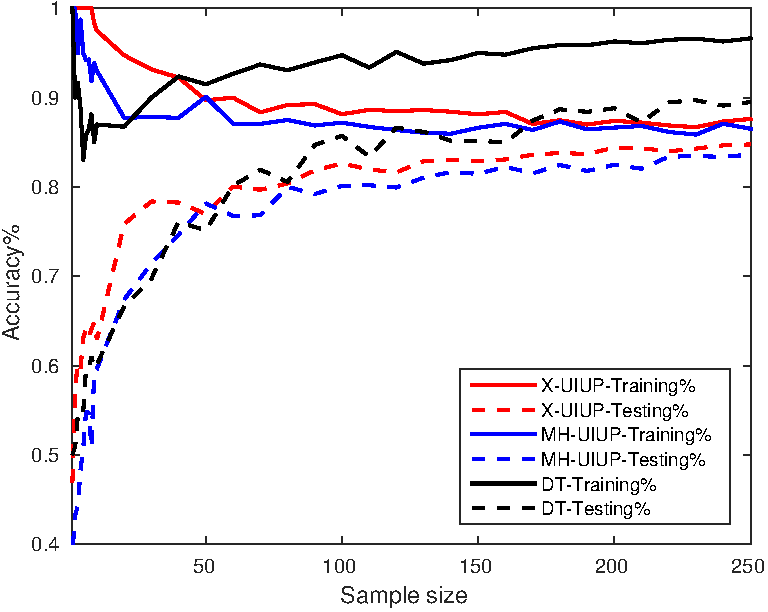
\includegraphics[width=\textwidth]{figs/PLPTF/Trees/CarEvaluation_Trees_X_MH.pdf}
  	\caption{CarEvaluation}
		\label{fig:Car1}
	\end{subfigure}
  \begin{subfigure}[b]{0.3\textwidth}
		\centering
  	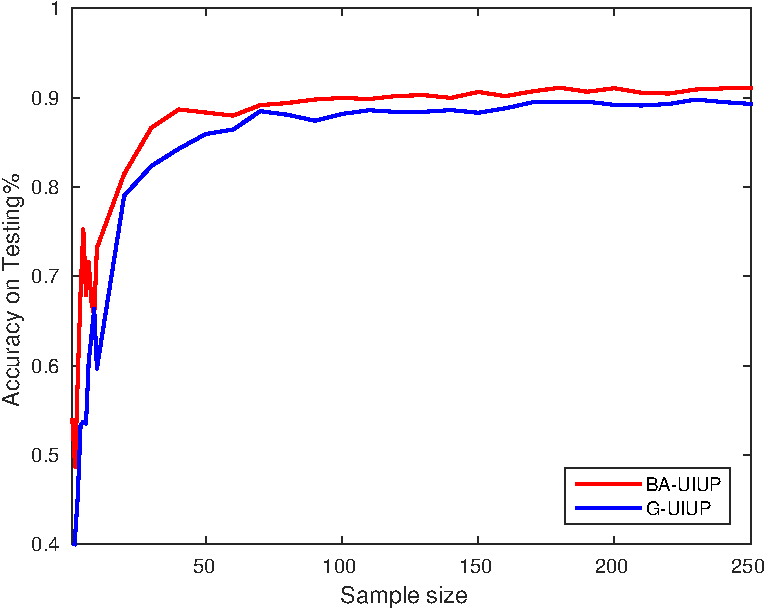
\includegraphics[width=\textwidth]{figs/PLPTF/Trees/CreditApprovalDownsampledFurther_Trees_X_MH.pdf}
  	\caption{CreditApproval}
		\label{fig:Crd1}
	\end{subfigure}
  \\
  \begin{subfigure}[b]{0.3\textwidth}
		\centering
  	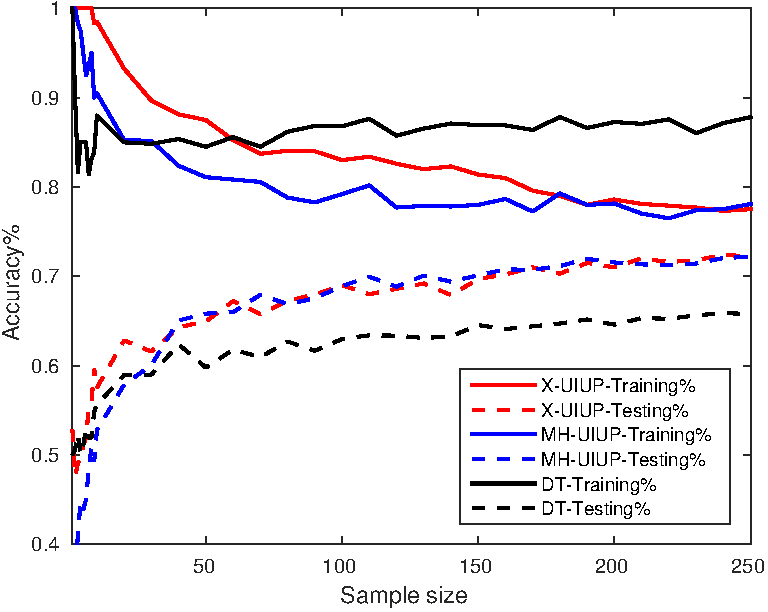
\includegraphics[width=\textwidth]{figs/PLPTF/Trees/GermanCreditDownsampledFurther_Trees_X_MH.pdf}
  	\caption{GermanCredit}
		\label{fig:G1}
	\end{subfigure}
  \begin{subfigure}[b]{0.3\textwidth}
		\centering
  	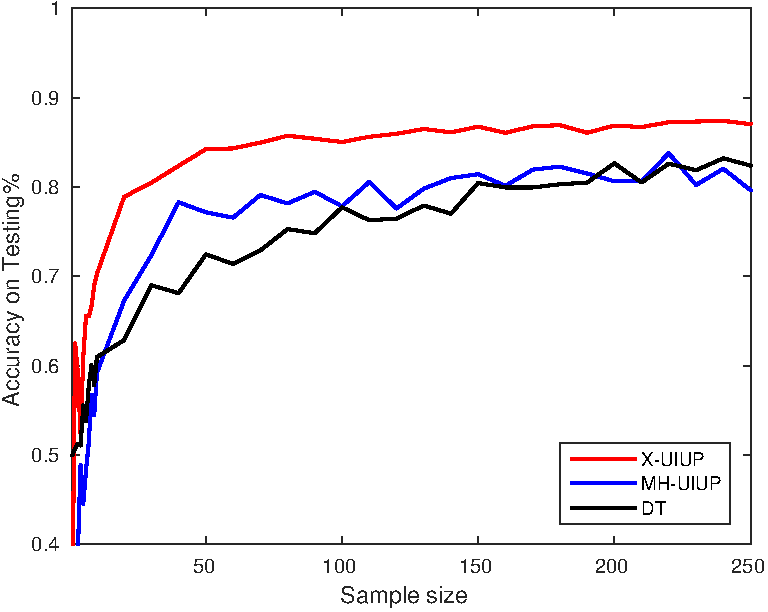
\includegraphics[width=\textwidth]{figs/PLPTF/Trees/IonosphereDownsampledFurther_Trees_X_MH.pdf}
  	\caption{Ionosphere}
		\label{fig:I1}
	\end{subfigure}
  \begin{subfigure}[b]{0.3\textwidth}
		\centering
  	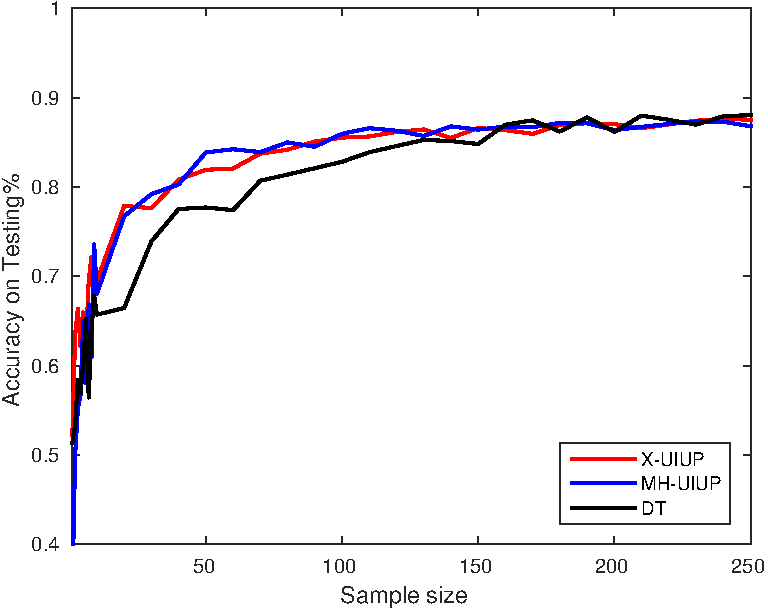
\includegraphics[width=\textwidth]{figs/PLPTF/Trees/MammographicMassDownsampled_Trees_X_MH.pdf}
  	\caption{MammographicMass}
		\label{fig:Mam1}
	\end{subfigure}
	\\
  \begin{subfigure}[b]{0.3\textwidth}
		\centering
  	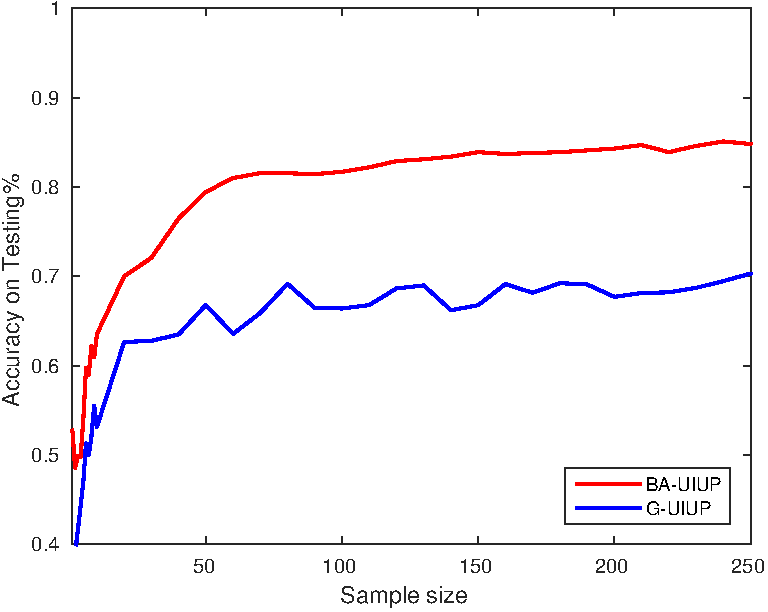
\includegraphics[width=\textwidth]{figs/PLPTF/Trees/MushroomDownsampled_Trees_X_MH.pdf}
  	\caption{Mushroom}
		\label{fig:Mush1}
	\end{subfigure}
  \begin{subfigure}[b]{0.3\textwidth}
		\centering
  	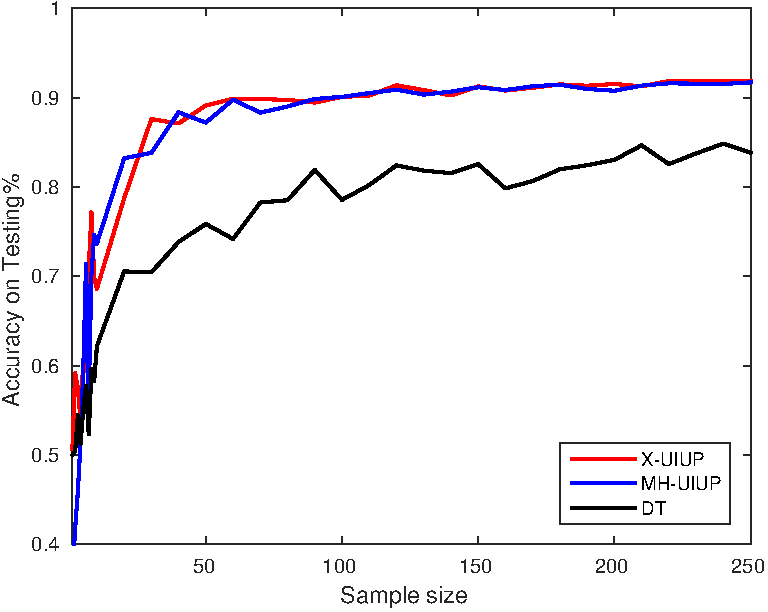
\includegraphics[width=\textwidth]{figs/PLPTF/Trees/NurseryDownsampledFurther_Trees_X_MH.pdf}
  	\caption{Nursery}
		\label{fig:N1}
	\end{subfigure}
  \begin{subfigure}[b]{0.3\textwidth}
		\centering
  	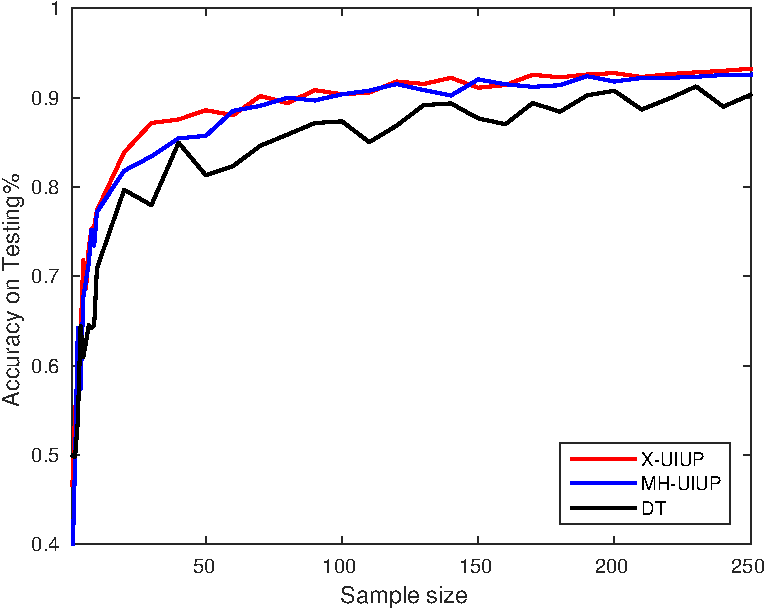
\includegraphics[width=\textwidth]{figs/PLPTF/Trees/SpectHeartDownsampledFurther_Trees_X_MH.pdf}
  	\caption{SPECTHeart}
		\label{fig:S1}
	\end{subfigure}
  \\
  \begin{subfigure}[b]{0.3\textwidth}
		\centering
  	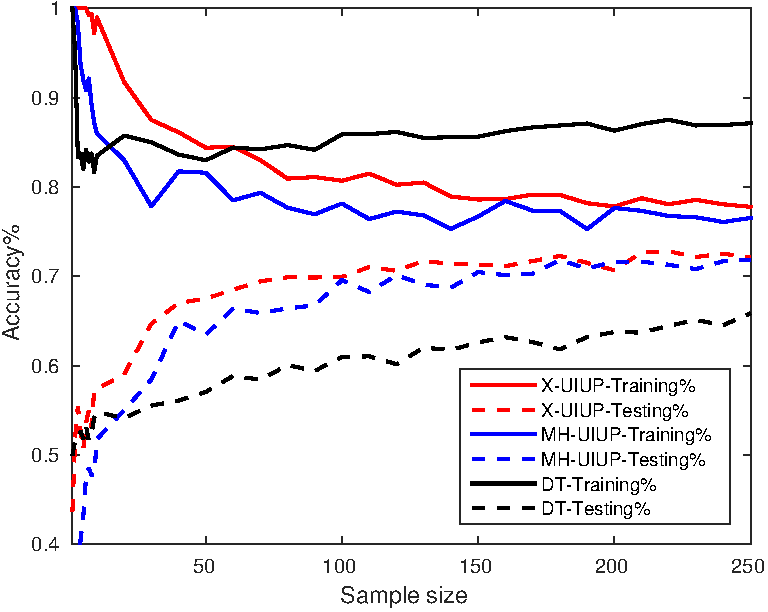
\includegraphics[width=\textwidth]{figs/PLPTF/Trees/TicTacToe_Trees_X_MH.pdf}
  	\caption{TicTacToe}
		\label{fig:T1}
	\end{subfigure}
  \begin{subfigure}[b]{0.3\textwidth}
		\centering
  	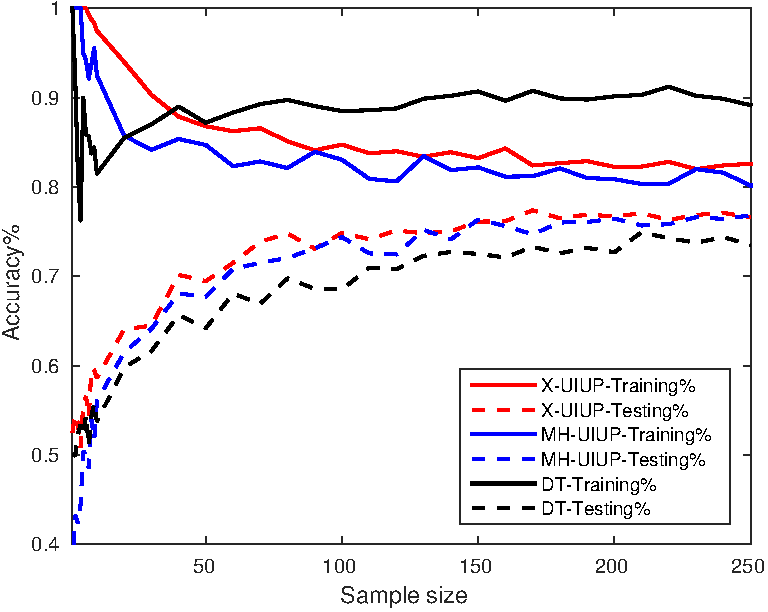
\includegraphics[width=\textwidth]{figs/PLPTF/Trees/VehicleDownsampledFurther_Trees_X_MH.pdf}
  	\caption{Vehicle}
		\label{fig:V1}
	\end{subfigure}
  \begin{subfigure}[b]{0.3\textwidth}
		\centering
  	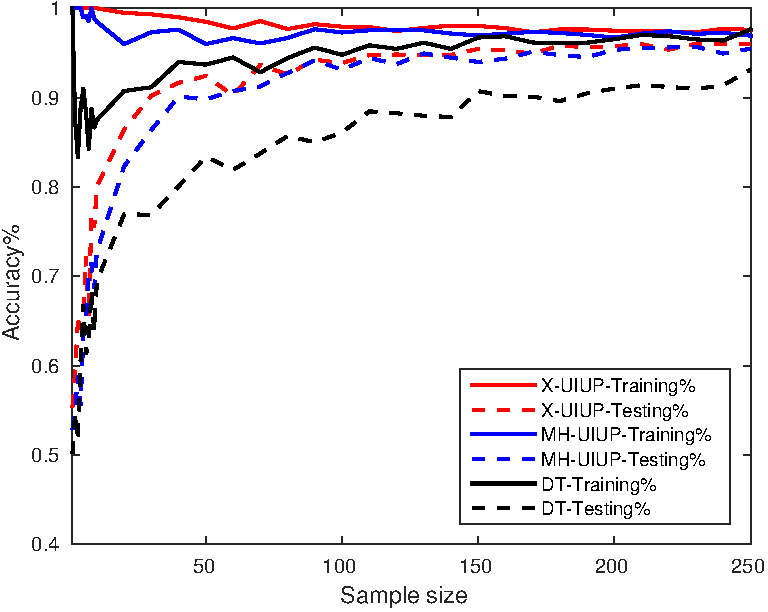
\includegraphics[width=\textwidth]{figs/PLPTF/Trees/WineDownsampled_Trees_X_MH.pdf}
  	\caption{Wine}
		\label{fig:W1}
	\end{subfigure}

  \caption{Learning UIUP PLP-trees}
  \label{fig:trees1}
\end{figure}

Since the best-agreement method quickly fails as the training sample size 
grows, in experiments with large learning sets we only used the greedy 
heuristics to learn PLP-trees from the classes UIUP, UICP-1, CIUP 
(including CIUPB and CIUPD), and CICP.
As demonstrated above, the greedy heuristic is a good alternative to the 
best-agreement method. For a dataset $D$, we generate $\TR_{D}\subset 
\cE^\succ$ as the training set, and use $\TE_D =\cE^\succ\setminus \TR_D$ 
as the testing set. We learn UIUP, UICP-1, CIUPB, CIUPD and CICP trees based on
$\TR_D$ 
%($1\%*|\cE^\succ| \leq |\TR_{\cE^\succ}| \leq 70\%*|\cE^\succ|$)
%and $\TE_{\cE^\succ}$ ($\TE_{\cE^\succ}=\cE^\succ \backslash \TR_{\cE^\succ}$) 
%for training and testing, respectively.
%From $\TR_{\cE^\succ}$ we train UIUP, UICP-1, CIUP and CICP trees
using the greedy heuristics, and then we test the the trees learned on
the testing set $\TE_D$, computing their accuracy. In \tblref{trees2}, we 
present results of accuracy on testing using 70\% of $\cE^\succ$
in the training phase. (As in the previous experiment, we computed the 
learning curves by varying the size of the training set up to 70\% of the 
size of $\cE^\succ$. The curves show similar behavior to those presented
earlier --- the accuracy increases with the size of the training set, but
gets close to the maximum accuracy already for relatively small training 
sets.) 

\begin{table}
  \centering
  \small
  \caption{Accuracy percents on the testing data (30\% of $\cE^\succ$)
					 for all four classes of PLP-trees, using models learned
					 by the greedy algorithm from the learning 
					 data (the other 70\% of $\cE^\succ$)}
	\setlength\tabcolsep{6pt}
  %\begin{tabular}{ |c||c|c|r@{ | }l|c| }
  \begin{tabular}{ |c||c|c|c|c|c| }
    \hline
    %Dataset          	 & UIUP & UICP-1 & \multicolumn{2}{c|}{CIUP[D|B]}     & CICP \\
    Dataset          	 & UIUP & UICP-1 & CIUPB & CIUPD & CICP \\
    \hline \hline                                             
    BreastCancerWisconsin                & 90.7 & 91.4   & 91.0  & 90.7  & 91.4   \\ \hline
    CarEvaluation                 & 85.8 & 86.0   & 85.8  & 85.9  & 86.0   \\ \hline
    CreditApproval                 & 91.4 & 91.7   & 91.6  & 92.0  & 92.2   \\ \hline
    GermanCredit                 & 74.3 & 74.6   & 74.3  & 74.5  & 75.7   \\ \hline
    Ionosphere                 & 87.1 & 86.9   & 87.2  & 88.5  & 90.4   \\ \hline
    MammographicMass                 & 88.2 & 89.5   & 87.3  & 86.9  & 90.0   \\ \hline
    Mushroom                 & 71.6 & 74.2   & 77.1  & 75.6  & 76.6   \\ \hline
    Nursery                 & 92.9 & 93.0   & 93.0  & 93.0  & 93.0   \\ \hline
    SPECTHeart                 & 93.4 & 94.9   & 95.4  & 94.8  & 95.7   \\ \hline
    TicTacToe                & 73.9 & 74.5   & 74.4  & 75.4  & 76.2   \\ \hline
    Vehicle                 & 79.2 & 80.4   & 80.3  & 80.0  & 81.2   \\ \hline
    Wine                 & 95.5 & 97.8   & 97.8  & 97.5  & 97.8   \\ \hline
    %WAvg               & 85.4 & 85.7   & 85.6  & 85.8  & 86.1   \\ \hline
  \end{tabular}
  \label{tbl:trees2}
\end{table}


%What we have learned from \tblref{trees2}:
%\begin{enumerate}
%	\item UIUP trees performs well, with all datasets above 70\%, and
%				4 datasets (GermanCredit,
%				Mushroom, TicTacToe and Vehicle) below 85\%.
%				Average accurracy for UIUP across all datasets is 85.3\%.
%	\item Average accurracy for UICP-1 across all datasets is 86.2\%.
%				UICP-1 trees outperforms UIUP trees on all but one dataset
%				Ionosphere.
%				Average improvement is 0.9 percentage points.
%	\item Average accurracy for CIUP across all datasets is 86.2\%.
%				CIUP trees outperforms UIUP trees on all but one dataset
%				MammographicMass.
%				Average improvement is 0.9 percentage points.
%	\item Average accurracy for CICP across all datasets is 87.2\%.
%				CICP trees outperforms all other classes of trees on all
%				datasets.
%				Average improvement is 1.9 percentage points.
%\end{enumerate}
From \tblref{trees2} we note that, for the greedy algorithm,
(1) for all datasets, there is a clear gain in the accuracies for 
the UIUP models using larger training sets;
(2) for all but one dataset (Ionosphere), the UICP-1 models, which allow for 
simple conditional preference statements, are more accurate than the UIUP 
models;
(3) both the CIUPB and CIUPD models are more accurate than the UIUP 
models for all but one dataset (MammographicMass); and
(4) the most general class CICP achieves the best accuracies among
all four classes of PLP-trees across all datasets.

The size of a PLP-tree is measured by the total number of preferences
in the CPTs in the tree.  Clearly, for UIUP, CIUP and CICP trees, it is
also the number of non-leaf nodes in the tree. For UICP trees it is the total
number of rows in all conditional preference tables in the tree. It is 
desirable to learn trees that are accurate but small. Trees of a small size 
provide insights into the structure and properties of the preference
order of a user.

The size of a PLP-tree learned by the greedy algorithm is bounded by
the number of training examples. On the other hand, it never exceeds 
the size of the largest possible tree for a domain it models. These 
maxima are shown for each dataset in \tblref{trees_max_size}.
The maximum
for CI trees is the common maximum for UICPB, UICPD and CICP trees.
The last column in the table shows the size of the training example set
used (70\% of all examples).
%Therefore, we want to compare the size of a learned tree with
%the smaller one of the two factors: the size of the training sample
%(denoted by $|\cE^\succ_\train|$, where $\cE^\succ_\train$
%contains 70\% of $\cE^\succ$) and
%the maximum size of any tree in the same class.
%We refer to \tblref{trees_max_size} for these two factors for all
%datasets and all classes of PLP-trees.
%Note that we replace three columns for UICPB, UICPD and CICP by
%one column for CI, because the data in all three columns are
%the same.
%From \tblref{trees_max_size}, we see that, for every dataset, 
%the maximal sizes of UI trees are much smaller than the sizes 
%$|\cE^\succ_\train|$ of 
%training samples, and that the maximal sizes of CI trees are larger
%than $|\cE^\succ_\train|$ for some datasets and smaller for
%the others.

\begin{table}
  \centering
  \small
  \caption{Maximum sizes of trees for all the classes and the 
					 training sample sizes for all datasets}
	\setlength\tabcolsep{6pt}
  \begin{tabular}{ |c||c|c|c|c| }
    \hline
    Dataset           & UIUP & UICP-1 & CI      & $|\cE^\succ_\train|$ \\
    \hline \hline                                 
    BreastCancerWisconsin               & 9    & 33     & 87,381   & 6,306   \\ \hline
    CarEvaluation                & 6    & 21     & 853      & 477,904 \\ \hline
    CreditApproval                & 10   & 37     & 91,477   & 46,255  \\ \hline
    GermanCredit                & 10   & 37     & 349,525  & 120,657 \\ \hline
    Ionosphere                & 10   & 19     & 1,023    & 2,430   \\ \hline
    MammographicMass                & 5    & 17     & 341      & 554     \\ \hline
    Mushroom                & 10   & 37     & 91,477   & 5,913   \\ \hline
    Nursery                & 8    & 29     & 7,765    & 383,644 \\ \hline
    SPECTHeart                & 10   & 19     & 1,023    & 2,237   \\ \hline
    TicTacToe               & 9    & 25     & 9,841    & 145,482 \\ \hline
    Vehicle                & 10   & 37     & 349,525  & 53,699  \\ \hline
    Wine                & 10   & 37     & 349,525  & 7,225   \\ \hline
    %Avg               & 8.9  & 29     & 111,646  & 104,359 \\ \hline
  \end{tabular}
  \label{tbl:trees_max_size}
\end{table}

\tblref{trees_size} shows average size of trees learned by our greedy 
algorithm (for each dataset and for each class of trees considered). The
results indicate that the learned trees have indeed relatively small sizes
when compared to the upper bounds implied by \tblref{trees_max_size}. The 
difference is drastic for CIUPB, CIUPD and CICP trees, where trees we learn
have sizes that are small fractions of the maximum possible size they 
potentially might have. For UIUP trees and UICP-1 trees, the difference is 
smaller (these trees because of their structure are very small to start with),
yet even there is some cases the learned trees have sizes below 80\% of the
maximum size and occasionally are much smaller (for instance for the Wine 
dataset). These small-size trees can provide explicit insights into the 
importance the user assigns to attributes when deciding between outcomes, and 
into how her preferences of attributes depend on preferences on the more 
important ones. 

We also observe that the sizes of learned CIUPB trees are always smaller 
than the sizes of the learned CI trees of the other two types. In some 
cases (datasets GermanCredit, Nursery, TicTacToe, Vehicle), they are significantly smaller. Given 
that the accuracies of learned CIUPB and CIUPD trees are very close to 
each other, and the accuracies of the learned CIUPB and CICP trees differ
by more than 2 percentage points in only one case (GermanCredit), the results suggests 
that CIUPB trees provide a a particularly attractive preference model.
The results are well aligned with the intuition that when using CIUP trees,
agents build them level by level in a breadth-first fashion.

%As a brief note on the two methods (depth-first and breadth-first)
%of learning CIUP PLP-trees,
%we observe from \tblref{trees2} and \tblref{trees_size} that
%CIUPB trees have less than half the size of CIUPD trees (31.0 vs 72.9),
%while obtaining almost the same accuracy (85.6 vs 85.8).
%This seems to suggest that the breadth-first method has
%the edge over the depth-first method when learning CIUP trees.
%It is aligned with our speculation that, when using CIUP trees,
%agents would rather make
%all the decisions at a level in a tree before moving to the lower
%one of less importance, than decide preferences along a path

%For UIUP trees, the They are smaller by up to size of  learns trees of relatively small 
%sizes. representations.
%We refer to \tblref{trees_size} for the average sizes of PLP-trees
%of various classes learned by the greedy algorithm from $\cE^\succ_\train$
%for all datasets.
%We see in \tblref{trees_size} that, across all classes of PLP-trees, 
%the greedy algorithms have learned reasonable-scale models (mostly 
%of size fewer than 100), in general much smaller than both the maximal
%possible sizes and the training sample sizes.
%For instance, for the Wine dataset, our algorithms have learn
%UIUP trees with size 5.1 compared to the upper-bound 10,
%UICP-1 trees with 13.3 to 37, CIUPB trees with 14.2
%to 7225, CIUPD trees with 16.9 to 7225, and
%CICP trees with 14.6 to 7225.
%This fact that our algorithms have learned partial trees
%provides valuable insights into the meaningful structures of the
%preference models: what attributes are useful and useless
%when making decisions, and which of the useful attributes
%are more important than others.

\begin{table}
  \centering
  \small
  \caption{Sizes of trees learned by the greedy algorithm from the training 
					 data (70\% of $\cE^\succ$)}
	\setlength\tabcolsep{6pt}
  %\begin{tabular}{ |c||c|c|r@{ | }l|c| }
  \begin{tabular}{ |c||c|c|c|c|c| }
    \hline
    %Dataset          & UIUP & UICP-1 & \multicolumn{2}{c|}{CIUP[D|B]}     & CICP \\
    Dataset          & UIUP & UICP-1 & CIUPB & CIUPD  & CICP \\
    \hline \hline                                       
    BreastCancerWisconsin              & 6.7  & 21.8   & 19.8  & 28.0   & 25.7    \\ \hline
    CarEvaluation               & 6.0  & 17.0   & 73.2  & 108.9  & 109.5   \\ \hline
    CreditApproval               & 9.0  & 24.7   & 31.3  & 78.6   & 81.1    \\ \hline
    GermanCredit               & 9.7  & 36.0   & 49.8  & 210.3  & 190.0   \\ \hline
    Ionosphere               & 9.6  & 17.2   & 19.8  & 31.5   & 30.6    \\ \hline
    MammographicMass               & 4.5  & 14.7   & 8.3   & 10.8   & 10.0    \\ \hline
    Mushroom               & 7.6  & 20.7   & 15.7  & 22.7   & 16.3    \\ \hline
    Nursery               & 8.0  & 25.7   & 56.2  & 121.0  & 116.9   \\ \hline
    SPECTHeart               & 8.4  & 13.7   & 13.0  & 18.4   & 19.0    \\ \hline
    TicTacToe              & 8.0  & 21.8   & 36.8  & 126.8  & 115.2   \\ \hline
    Vehicle               & 9.0  & 32.7   & 33.9  & 101.3  & 105.4   \\ \hline
    Wine               & 5.1  & 13.3   & 14.2  & 16.9   & 14.6    \\ \hline
    %Avg              & 7.6  & 21.6   & 31.0  & 72.9   & 69.5    \\ \hline
  \end{tabular}
  \label{tbl:trees_size}
\end{table}

Another important observation concerning our greedy algorithms is that
they work fast even on large training sets. This is demonstrated in 
\figref{trees_time}, where we show the effectiveness of the greedy method
for datasets BreastCancerWisconsin and Vehicle, and contrast it with highly limited range of
applicability of the best-agreement method. For other datasets, we observe 
a similar behavior.

\begin{figure}
	\centering

  \begin{subfigure}[b]{0.45\textwidth}
		\centering
  	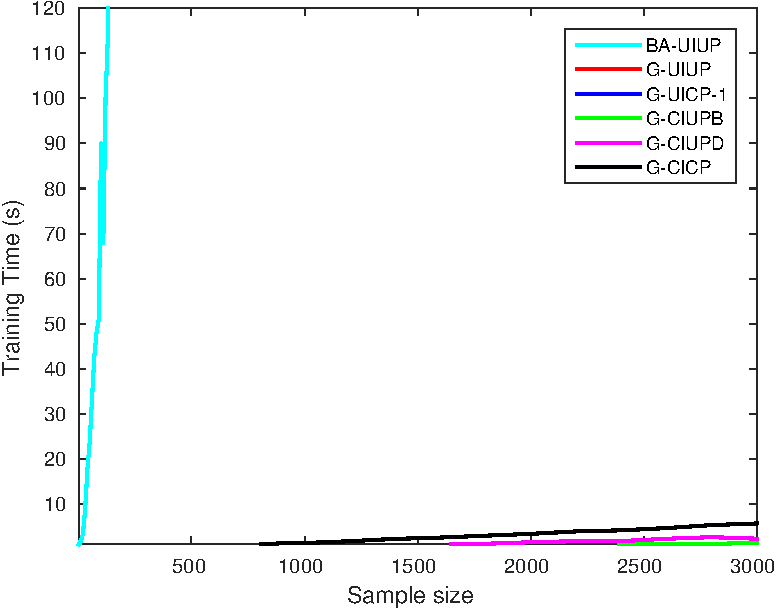
\includegraphics[width=\textwidth]{figs/PLPTF/Time/Trees/BreastCancerWisconsinDownsampled.pdf}
  	\caption{BreastCancerWisconsin}
		\label{fig:BreastCancerWisconsin_T}
	\end{subfigure}
  \begin{subfigure}[b]{0.45\textwidth}
		\centering
  	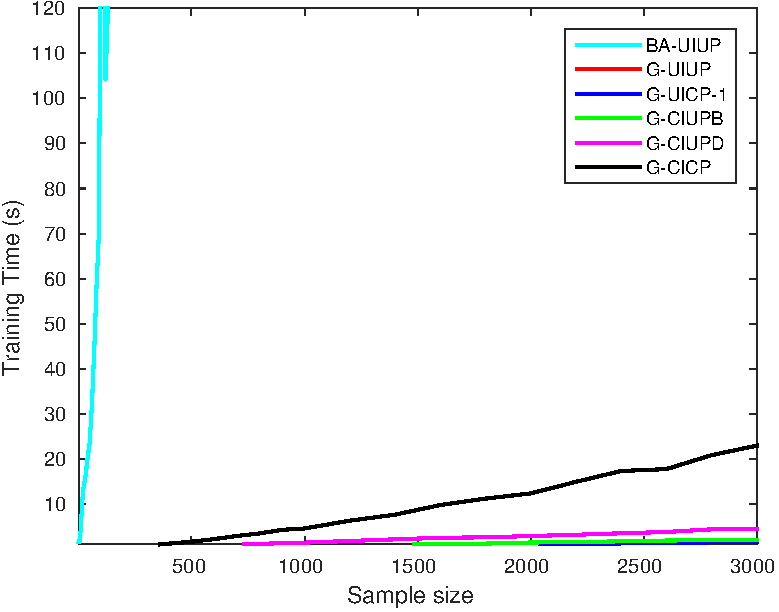
\includegraphics[width=\textwidth]{figs/PLPTF/Time/Trees/VehicleDownsampledFurther.pdf}
  	\caption{Vehicle}
		\label{fig:Vehicle_T}
	\end{subfigure} 

  \caption{Training time comparison: best-agreement vs. greedy}
  \label{fig:trees_time}
\end{figure}

%\begin{figure}[ht]
%	\centering
%
%  \begin{subfigure}[b]{0.3\textwidth}
%		\centering
%		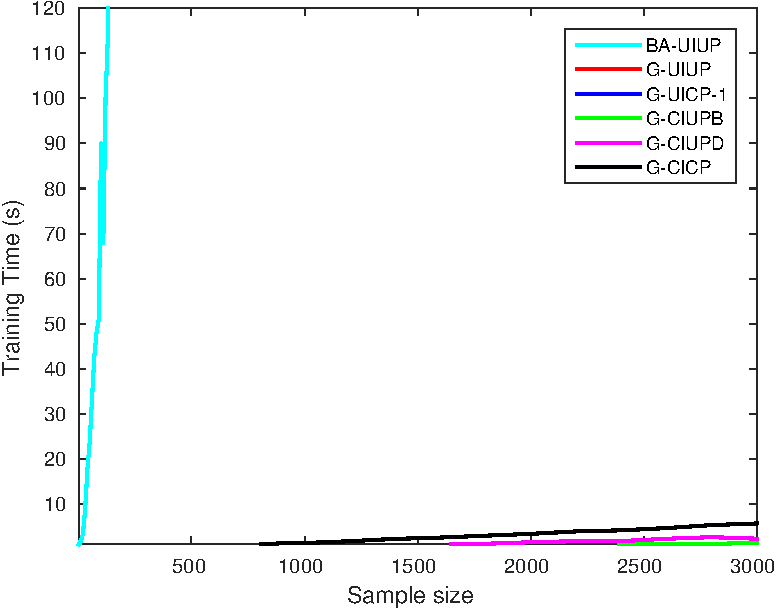
\includegraphics[width=\textwidth]{figs/PLPTF/Time/Trees/BreastCancerWisconsinDownsampled.pdf}
%		\caption{BreastCancerWisconsin}
%		\label{fig:B_Time}
%	\end{subfigure}
%  \begin{subfigure}[b]{0.3\textwidth}
%		\centering
%  	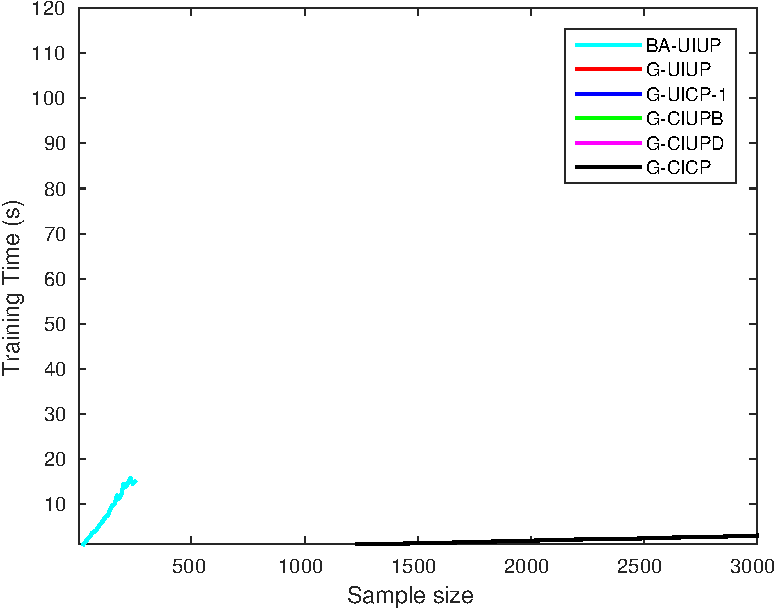
\includegraphics[width=\textwidth]{figs/PLPTF/Time/Trees/CarEvaluation.pdf}
%  	\caption{CarEvaluation}
%		\label{fig:Car_Time}
%	\end{subfigure}
%  \begin{subfigure}[b]{0.3\textwidth}
%		\centering
%  	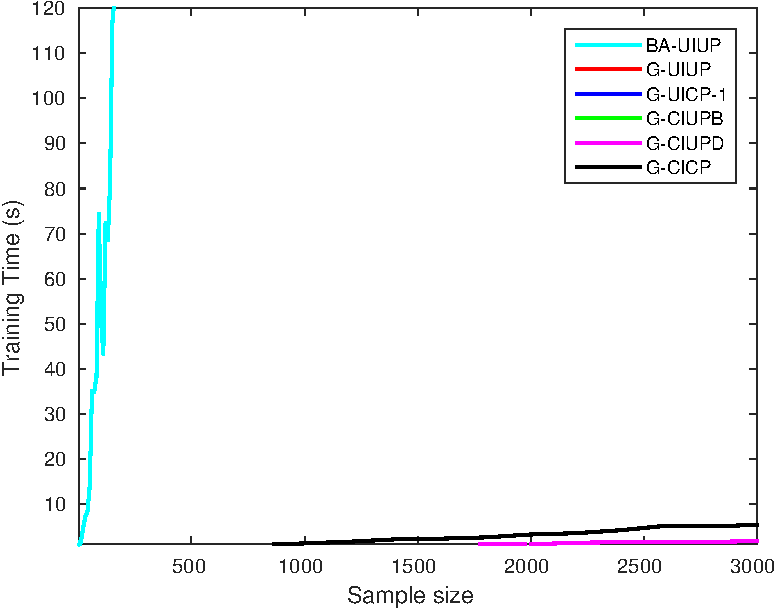
\includegraphics[width=\textwidth]{figs/PLPTF/Time/Trees/CreditApprovalDownsampledFurther.pdf}
%  	\caption{CreditApproval}
%		\label{fig:Crd_Time}
%	\end{subfigure}
%  \\
%  \begin{subfigure}[b]{0.3\textwidth}
%		\centering
%  	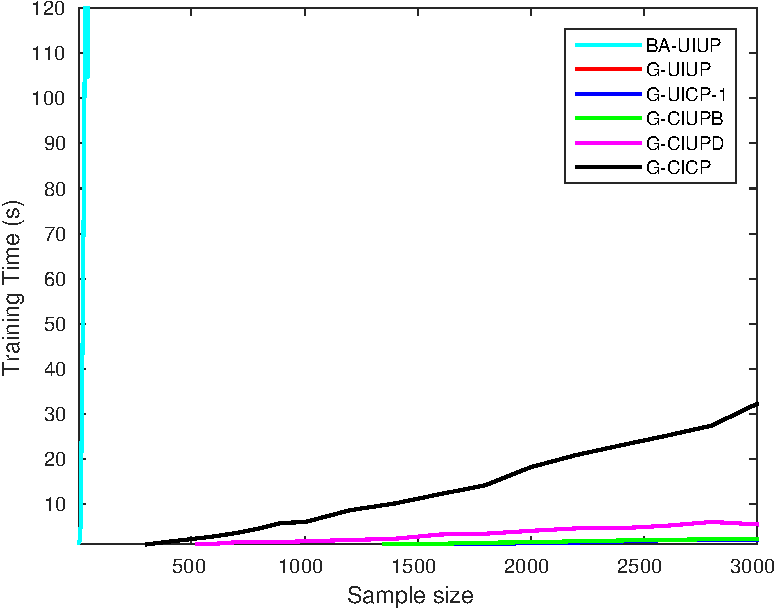
\includegraphics[width=\textwidth]{figs/PLPTF/Time/Trees/GermanCreditDownsampledFurther.pdf}
%  	\caption{GermanCredit}
%		\label{fig:G_Time}
%	\end{subfigure}
%  \begin{subfigure}[b]{0.3\textwidth}
%		\centering
%  	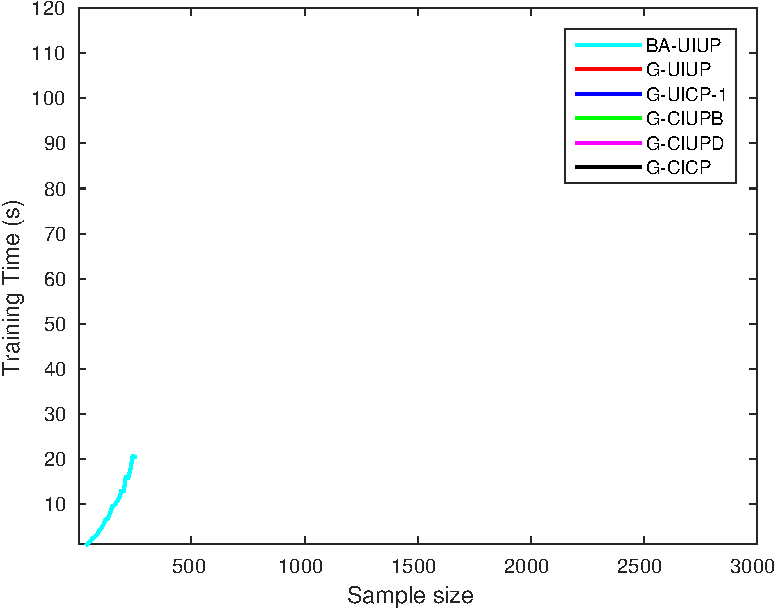
\includegraphics[width=\textwidth]{figs/PLPTF/Time/Trees/IonosphereDownsampledFurther.pdf}
%  	\caption{Ionosphere}
%		\label{fig:I_Time}
%	\end{subfigure}
%  \begin{subfigure}[b]{0.3\textwidth}
%		\centering
%  	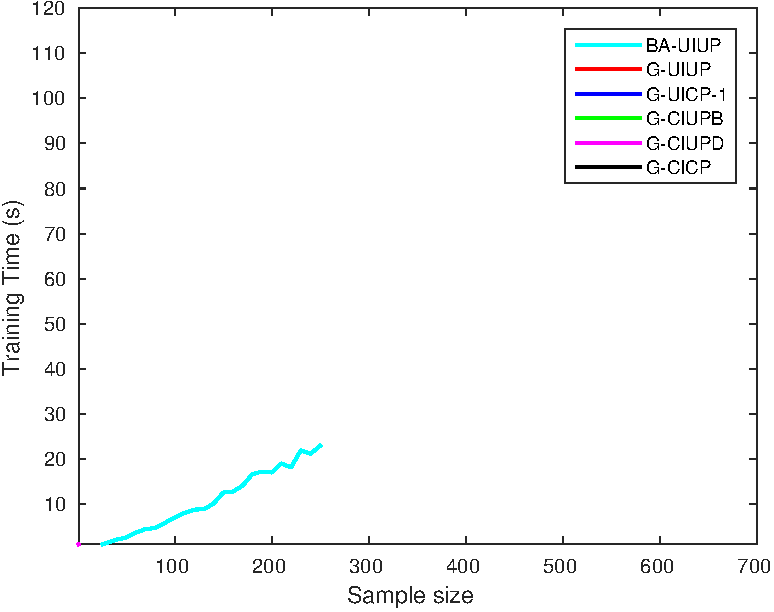
\includegraphics[width=\textwidth]{figs/PLPTF/Time/Trees/MammographicMassDownsampled.pdf}
%  	\caption{MammographicMass}
%		\label{fig:Mam_Time}
%	\end{subfigure}
%	\\
%  \begin{subfigure}[b]{0.3\textwidth}
%		\centering
%  	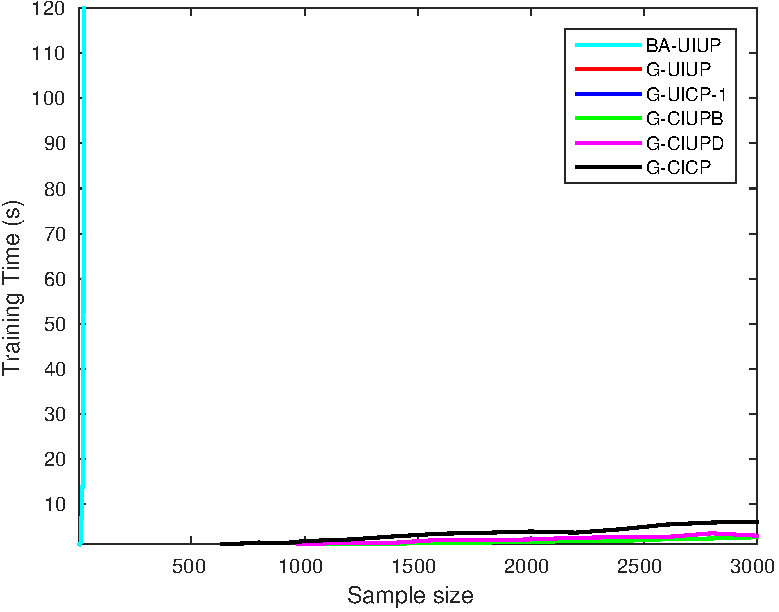
\includegraphics[width=\textwidth]{figs/PLPTF/Time/Trees/MushroomDownsampled.pdf}
%  	\caption{Mushroom}
%		\label{fig:Mush_Time}
%	\end{subfigure}
%  \begin{subfigure}[b]{0.3\textwidth}
%		\centering
%  	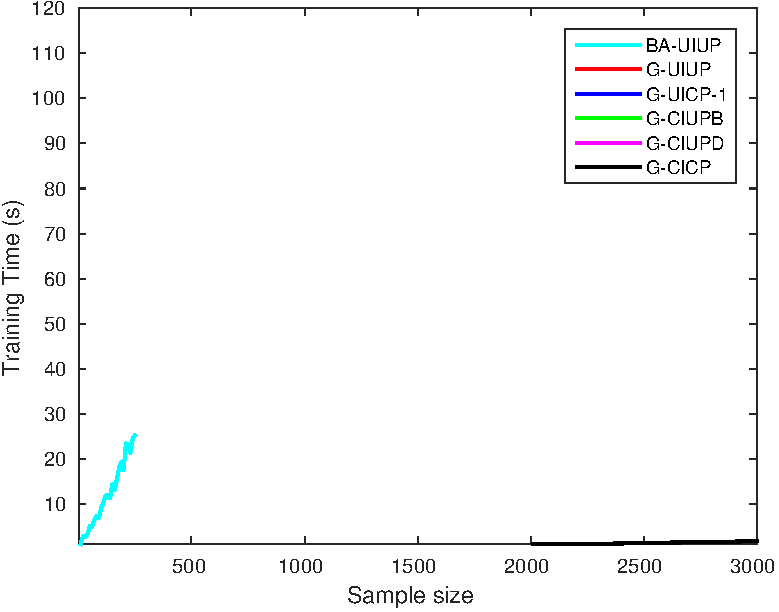
\includegraphics[width=\textwidth]{figs/PLPTF/Time/Trees/NurseryDownsampledFurther.pdf}
%  	\caption{Nursery}
%		\label{fig:N_Time}
%	\end{subfigure}
%  \begin{subfigure}[b]{0.3\textwidth}
%		\centering
%  	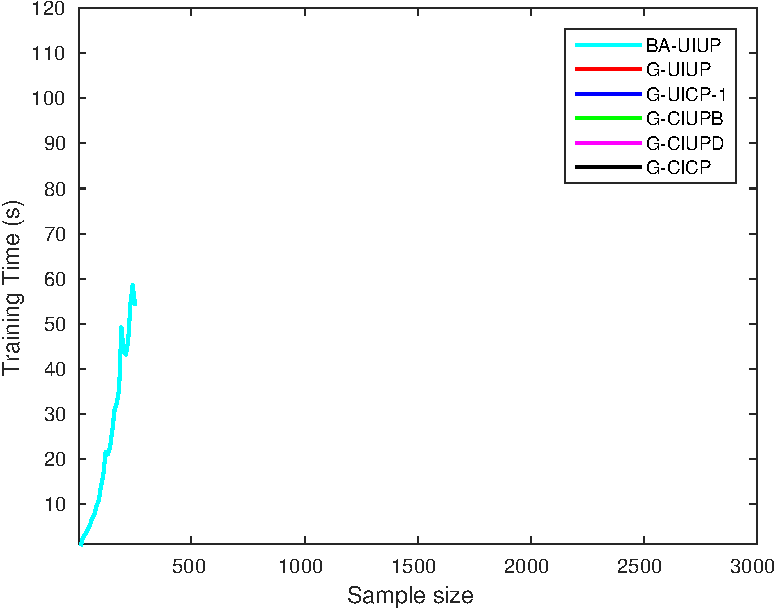
\includegraphics[width=\textwidth]{figs/PLPTF/Time/Trees/SpectHeartDownsampledFurther.pdf}
%  	\caption{SPECTHeart}
%		\label{fig:S_Time}
%	\end{subfigure}
%  \\
%  \begin{subfigure}[b]{0.3\textwidth}
%		\centering
%  	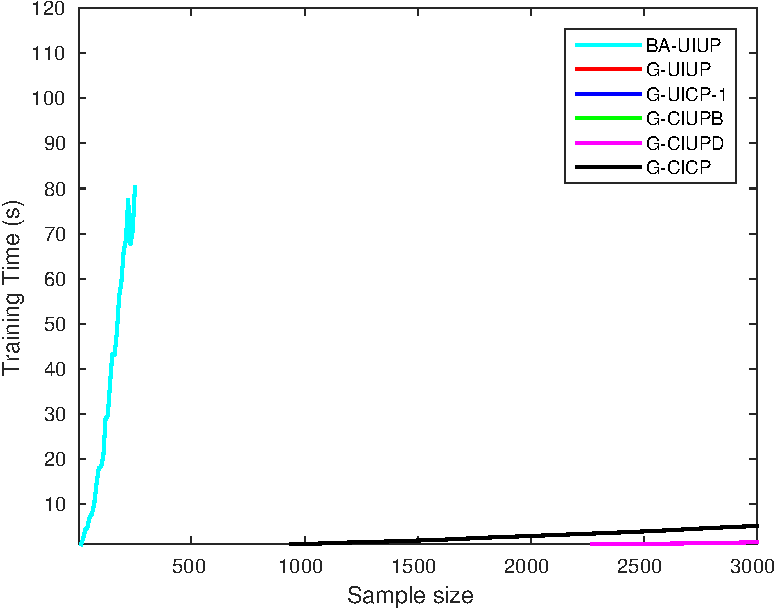
\includegraphics[width=\textwidth]{figs/PLPTF/Time/Trees/TicTacToe.pdf}
%  	\caption{TicTacToe}
%		\label{fig:T_Time}
%	\end{subfigure}
%  \begin{subfigure}[b]{0.3\textwidth}
%		\centering
%  	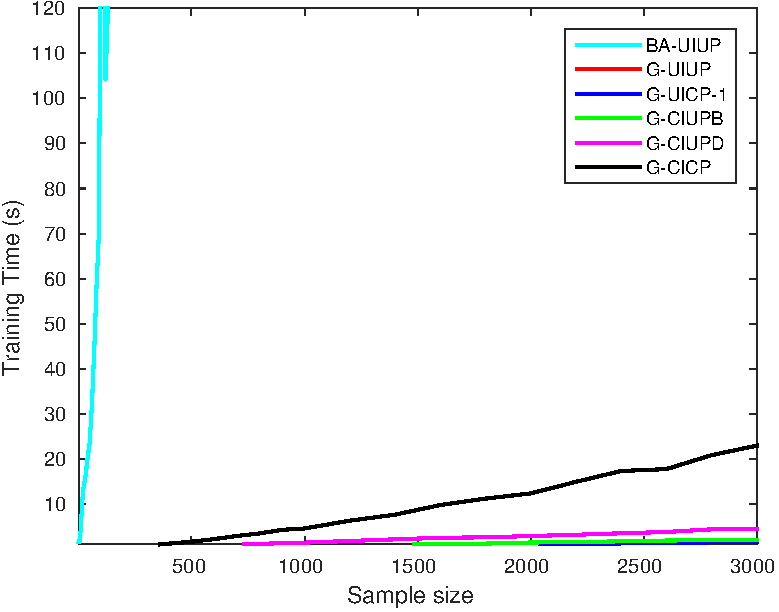
\includegraphics[width=\textwidth]{figs/PLPTF/Time/Trees/VehicleDownsampledFurther.pdf}
%  	\caption{Vehicle}
%		\label{fig:V_Time}
%	\end{subfigure}
%  \begin{subfigure}[b]{0.3\textwidth}
%		\centering
%  	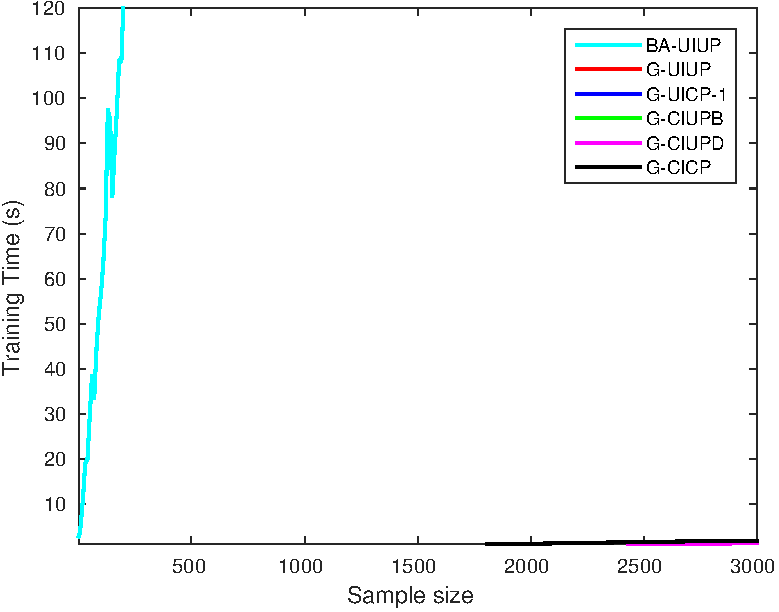
\includegraphics[width=\textwidth]{figs/PLPTF/Time/Trees/WineDownsampled.pdf}
%  	\caption{Wine}
%		\label{fig:W4}
%	\end{subfigure}
%
%  \caption{Training time comparison: best-agreement vs. greedy}
%  \label{fig:trees_time}
%\end{figure}

Closing this section, we provide a brief comparison between PLP-trees
and decision trees, a commonly-used classification model in machine learning.
Decision trees can be used as classifiers that, given two outcomes, can
tell if an outcome is better or worse than another.
Our experimental results show that decision trees are generally better than
PLP-trees, although the difference is mostly within 3 percentage points, 
on predicting
preferences between outcomes in the testing phase.
However, PLP-trees offer not only a quick way to determine dominance (the order
between two outcomes) but also insights into the structure of the reasoning 
process of the decision maker. They point to importance of attributes and
conditional dependencies between them, and explicitly identify optimal
outcomes. This information is hard to glean out of the decision-tree model 
for the dominance relation.  


\section{Partial Lexicographic Preference Forests}
\label{sec:forests}
As we see from \tblref{trees2}, our approximation method
achieves high accuracy (above 85\%) on most of the datasets
for all four types of PLP-trees. However, on some datasets such as Mushroom,
PLP-trees that we learn have accuracy below 80\% across all classes of trees.
In an effort to improve on this, we introduce the notion of a
\tit{PLP-forest}, that is, a \emph{collection} of PLP-trees.
Let $F= \{T_1,\ldots,T_n\}$ be a PLP-forest. We say that $F$ is a 
$\cC$ PLP-forest, where $\cC$ is one of the four classes UIUP, UICP-1, 
CIUP and CICP, if $F$ consists exclusively of $\cC$ PLP-trees. 

\subsection{Aggregating PLP-Trees in a PLP-Forest}
We use the \tit{pairwise majority rule} (PMR) to aggregate
orders defined by trees in a forest. 
%in order to make decisions 
%between pairs of outcomes in the testing phase.
The choice of PMR as the aggregation rule is motivated by three considerations.
First, plurality was used in the related
work on random forest learning that motivated and influenced our ideas behind
PLP forests and PLP forest learning. 
Second, the task we have at hand is to determine the preferences between
outcomes, so PMR is well aligned with this task (the outcome that ``wins''
on more orders ``wins'' overall). 
Finally, the PMR is intuitive and easy to implement.

Let us denote by $N_F(o_1,o_2)=|\{T \in F:o_1 \succ_T o_2\}|$
the number of trees in the forests where the outcome $o_1$ is
preferred to the outcome $o_2$.
%Now consider the dominance testing problem.
Given a forest $F$, and two outcomes $o_1$ and $o_2$,
we say that $o_1 \succ_F^\PMR o_2$ iff $N_F(o_1,o_2)>N_F(o_2,o_1)$,
and that $o_1 \approx_F^\PMR o_2$ iff $N_F(o_1,o_2)=N_F(o_2,o_1)$.

In some cases, PMR may lead to the so-called 
\tit{Condorcet's Paradox}, where the strict $\succ_F^\PMR$ 
relation contains a cycle.
%However, because it never happens that an outcome is preferred to itself in
%our datasets, Condorcet paradox is not the case for our datasets.
Earlier empirical studies, however, conclude that there is little evidence for
occurrences of Condorcet's Paradox.
Among these studies, one recent work by Mattei et al.
on the Netflix dataset showed that the Condorcet's Paradox
has a low occurrence percentage of less than 0.11\%\cite{mattei2012empirical}; 
that is, on average, out of one thousand elections they ran 
there was about one election where Condorcet's Paradox accrued.
Aligned with this empirical conclusion, our datasets are created 
in a way that Condorcet's Paradox is prevented from happening.
Other possible aggregators are positional
scoring rules (adjusted for total \tit{preorders}), Copeland's
method, among others.
We will leave this and discuss it later in the chapter as part of 
the future work.


\subsection{Experimentation}
To further boost up performances, we now show empirical results
of learning \tit{PLP-forests}.

First, we show results for UIUP PLP-forests using the best-agreement learning
and the greedy heuristics.
In each experiment, we randomly partition a dataset into training
set (70\%) and testing set (30\%), learn a forest of 5000 trees, where
each tree is learned from 50 randomly selected examples from the
training set, and then test the forest against the testing set.
We repeat it 20 times and report the average accuracy.
%Note that the plots also include a straight line representing
%the result for learning a UIUP PLP-tree, had we used all the
%training data to learn a single tree using the greedy heuristic.
We present these results in \tblref{forests1} (we write BA and G to indicate the method used).

\begin{table}
  \centering
  \small
  \caption{Accuracy percents on the testing data (30\% of $\cE^\succ$)
					 for UIUP trees and forests of 5000 UIUP trees, 
					 using the greedy and the best-agreement algorithms from the learning 
					 data (the other 70\% of $\cE^\succ$)}
  \begin{tabular}{ |c||c|c|c| }
    \hline
    Dataset          & G+Tree & G+Forest & BA+Forest\\
    \hline \hline
    BreastCancerWisconsin              & 90.7   & 93.4     & 95.1 \\ \hline
    CarEvaluation               & 85.8   & 91.9     & 89.2 \\ \hline      
    CreditApproval               & 91.4   & 91.5     & 93.1 \\ \hline       
    GermanCredit               & 74.3   & 75.4     & 77.9 \\ \hline     
    Ionosphere               & 87.1   & 83.0     & 92.5 \\ \hline   
    MammographicMass               & 88.2   & 89.1     & 90.8 \\ \hline         
    Mushroom               & 71.6   & 78.8     & 90.2 \\ \hline 
    Nursery               & 92.9   & 93.2     & 94.0 \\ \hline
    SPECTHeart               & 93.4   & 93.7     & 94.9 \\ \hline   
    TicTacToe              & 73.9   & 75.1     & 77.2 \\ \hline 
    Vehicle               & 79.2   & 82.7     & 81.9 \\ \hline
    Wine               & 95.5   & 95.8     & 96.9 \\ \hline
    %WAvg             & 85.4   & 88.3     & 88.1 \\ \hline
  \end{tabular}
  \label{tbl:forests1}
\end{table}

%What we have learned from \tblref{forests1}:
%\begin{enumerate}
%	\item UIUP forests using the greedy method
%				outperforms UIUP trees using the greedy method on all
%				but one dataset: Ionosphere.
%				Average improvement is 2.9 percentage points.
%	\item UIUP forests using the exact algorithm
%				outperforms UIUP trees using the greedy method on all
%				datasets.
%				Average improvement is 2.7 percentage points.
%	\item UIUP forests using the exact algorithm
%				outperforms UIUP forests using the greedy method on all
%				but two datasets: CarEvaluation and Vehicle.
%				Average improvement is 0.2 percentage points.
%\end{enumerate}

We see that G+Forest outperforms G+Tree on all but one
dataset (i.e., Ionosphere). This indicates the gain of using a forest of 
diverse trees against a single tree for UIUP.
Similarly, we observe that BA+Forest outperforms G+Forest on all
datasets but one (CarEvaluation). This points to another advantage of PLP forest
learning: they achieve good accuracy even when individual trees are learned
from small example sets and so, the best-agreement learning becomes practical.

Second, we show results for the greedy heuristics and the five types of 
PLP-forests (under the same setting as before).
% using the greedy heuristic for different sizes of forests.
%The experiment settings are similar to those described previously.
%Let us look at the accuracy results in \tblref{forests2} for different types of
%forests of 5000 trees learned by the greedy algorithm from
%small samples, again, of 50 examples.
%These results are shown in \figref{B4}, \figref{Car4}, \figref{Crd4}, \figref{I4},
%\figref{Mam4}, \figref{S4}, \figref{T4}, \figref{V4}, and \figref{W4}.

\begin{table}
  \centering
  \small
  \caption{Accuracy percents on the testing data (30\% of $\cE^\succ$)
					 for all four classes of PLP-forests of 5000 trees, 
					 using the greedy algorithm from the learning 
					 data (the other 70\% of $\cE^\succ$)}
  %\begin{tabular}{ |c||c|c|r@{ | }l|c| }
  \begin{tabular}{ |c||c|c|c|c|c| }
    \hline
    Dataset          				 & UIUP & UICP-1 & CIUPB & CIUPD & CICP \\
    \hline \hline                                              
    BreastCancerWisconsin                      & 93.4 & 94.1   & 93.7  & 94.1  & 94.0 \\ \hline
    CarEvaluation                       & 91.9 & 88.3   & 91.4  & 89.7  & 91.4 \\ \hline
    CreditApproval                       & 91.5 & 91.6   & 92.8  & 92.9  & 93.0 \\ \hline 
    GermanCredit                       & 75.4 & 73.8   & 76.1  & 76.1  & 76.2 \\ \hline     
    Ionosphere                       & 83.0 & 87.9   & 89.3  & 89.4  & 89.5 \\ \hline   
    MammographicMass                       & 89.1 & 90.1   & 90.0  & 90.1  & 90.2 \\ \hline         
    Mushroom                       & 78.8 & 87.2   & 92.2  & 92.2  & 91.8 \\ \hline 
    Nursery                       & 93.2 & 89.9   & 93.3  & 93.4  & 93.4 \\ \hline
    SPECTHeart                       & 93.7 & 93.5   & 93.6  & 93.6  & 93.7 \\ \hline   
    TicTacToe                      & 75.1 & 75.2   & 76.6  & 76.5  & 76.9 \\ \hline 
    Vehicle                       & 82.7 & 81.8   & 83.2  & 83.2  & 83.4 \\ \hline
    Wine                       & 95.8 & 95.4   & 97.5  & 97.8  & 97.8 \\ \hline
    %WAvg                     & 88.3 & 85.8   & 88.5  & 87.9  & 88.6 \\ \hline
  \end{tabular}
  \label{tbl:forests2}
\end{table}

The results are shown in \tblref{forests2}. Comparing with \tblref{trees2},
we see that UICP-1 trees do not lend themselves well to the use in forests,
the accuracies for individual UICP-1 trees are higher than for forests of
UICP-1 trees for five out of 12 datasets. However, for all other types of
trees, the idea of learning forests of such trees is very effective. We get
improvements in the accuracy on all datasets but one for UIUP and CIUPD
trees, and in all but two datasets for CIUPB and CICP trees. In the case 
of the dataset Mushroom, the improvements provided by forest learning are 
particularly significant.
%using them as members othe weighted average of accuracies across
%all types of PLP-forests are better than those for corresponding type
%of PLP-trees.
%For the Mushroom dataset, this improvement is rather significant, with
%7.2, 13, 15.1, 16.6, and 15.2 percentage points for the five classes, respectively.
%We also see that next to CICP with the highest average accuracy is class
%UIUP with only 0.3\% worse.
%This demonstrates that, thanks to the aggregating rule PMR, UIUP forests 
%generalize better to the testing data than UICP-1, CIUPB and CIUPD forests,
%whereas UIUP trees are outperformed by classes UICP-1, CIUPB and CIUPD.

We also studied how the accuracy of PLP-forests changes with the number of
their PLP-trees. In \figref{forests2}, we show the results for UIUP and CICP 
PLP-forests for all twelve datasets.

%\begin{figure}
%	\centering
%
%  \begin{subfigure}[b]{0.23\textwidth}
%		\centering
%  	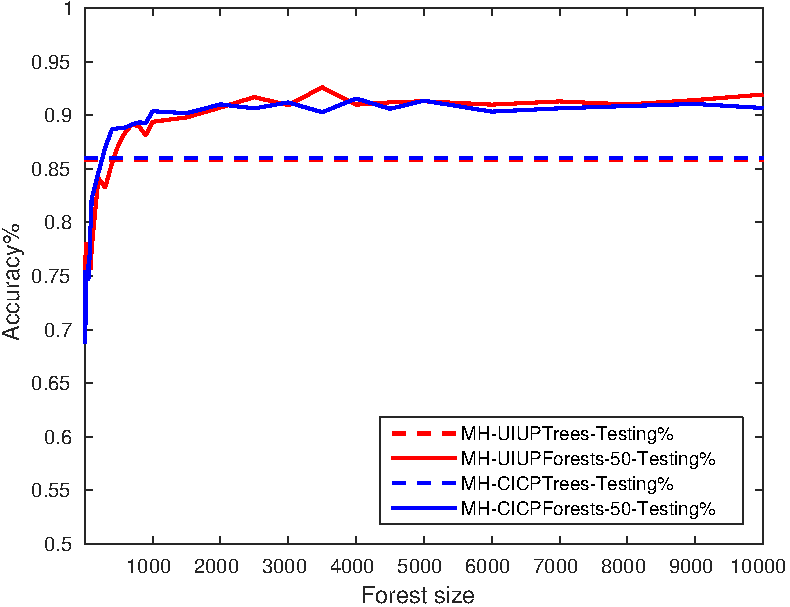
\includegraphics[width=\textwidth]{figs/PLPTF/Forests/CarEvaluation_Forests_MH.pdf}
%  	\caption{CarEvaluation}
%		\label{fig:Car4}
%	\end{subfigure}
%  \begin{subfigure}[b]{0.23\textwidth}
%		\centering
%  	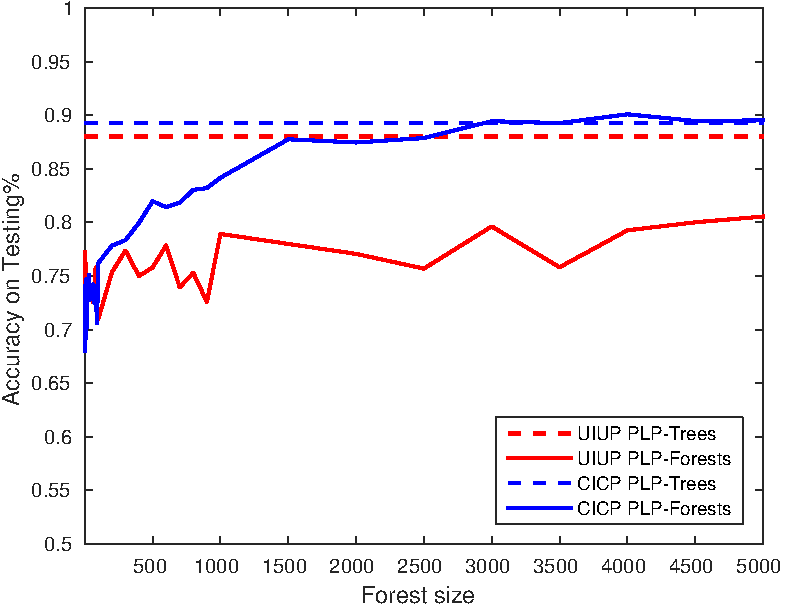
\includegraphics[width=\textwidth]{figs/PLPTF/Forests/IonosphereDownsampledFurther_Forests_MH.pdf}
%  	\caption{Ionosphere}
%		\label{fig:I4}
%	\end{subfigure}
%	\\
%  \begin{subfigure}[b]{0.23\textwidth}
%		\centering
%  	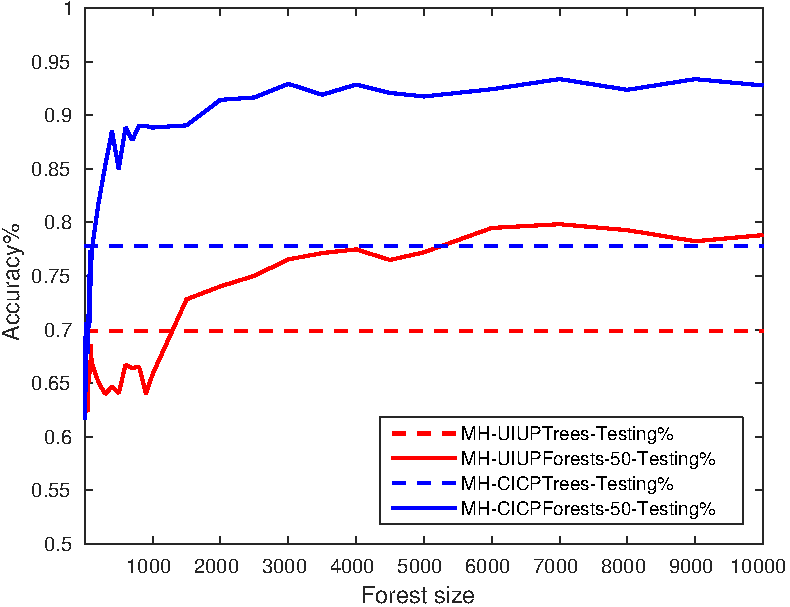
\includegraphics[width=\textwidth]{figs/PLPTF/Forests/MushroomDownsampled_Forests_MH.pdf}
%  	\caption{Mushroom}
%		\label{fig:Mush4}
%	\end{subfigure}
%  \begin{subfigure}[b]{0.23\textwidth}
%		\centering
%  	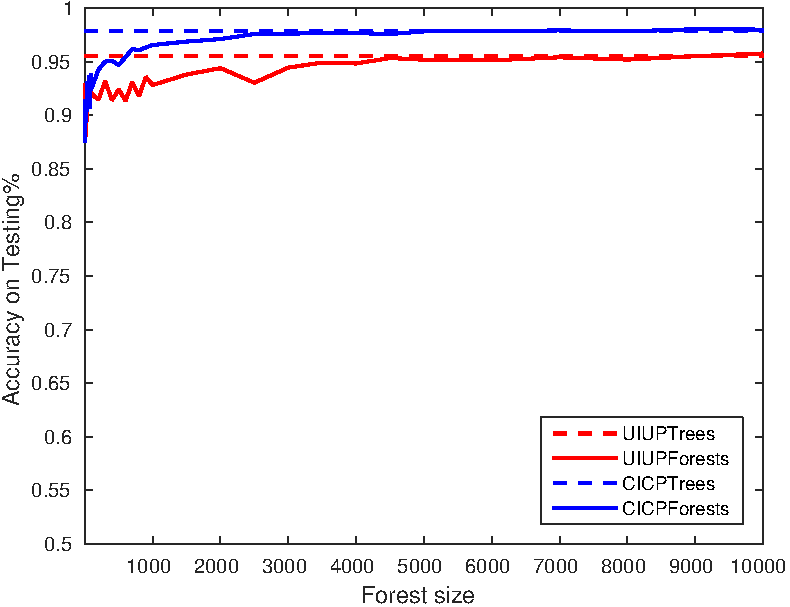
\includegraphics[width=\textwidth]{figs/PLPTF/Forests/WineDownsampled_Forests_MH.pdf}
%  	\caption{Wine}
%		\label{fig:W4}
%	\end{subfigure}
%
%  \caption{Learning PLP-forests}
%  \label{fig:forests2}
%\end{figure}

\begin{figure}[ht]
	\centering

  \begin{subfigure}[b]{0.3\textwidth}
		\centering
		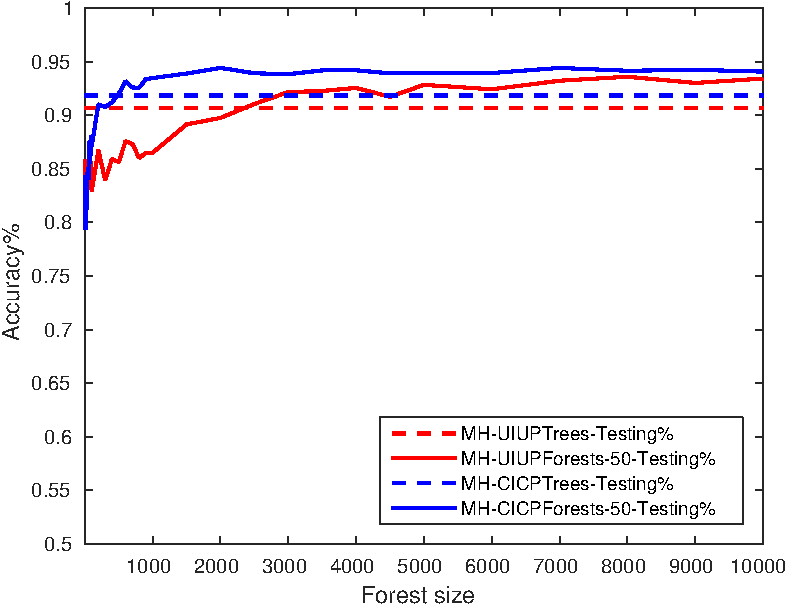
\includegraphics[width=\textwidth]{figs/PLPTF/Forests/BreastCancerWisconsinDownsampled_Forests_MH.pdf}
		\caption{BreastCancerWisconsin}
		\label{fig:B4}
	\end{subfigure}
  \begin{subfigure}[b]{0.3\textwidth}
		\centering
  	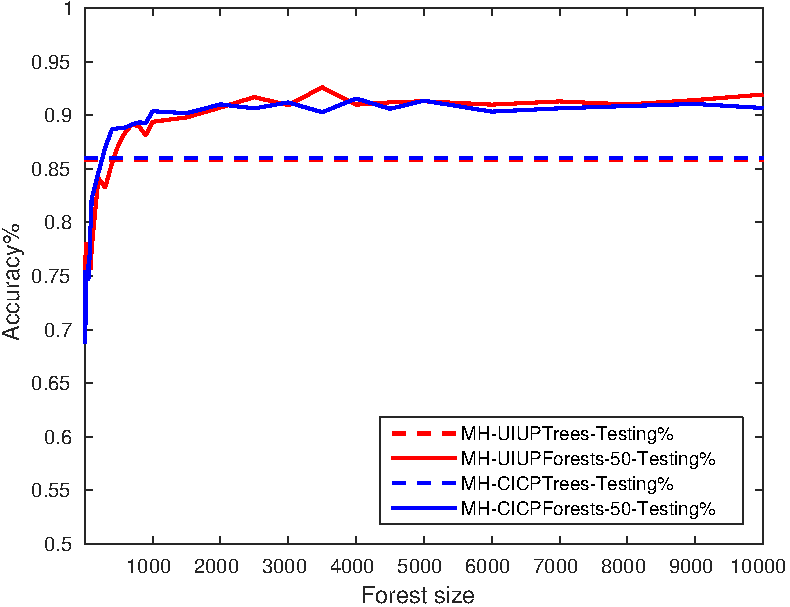
\includegraphics[width=\textwidth]{figs/PLPTF/Forests/CarEvaluation_Forests_MH.pdf}
  	\caption{CarEvaluation}
		\label{fig:Car4}
	\end{subfigure}
  \begin{subfigure}[b]{0.3\textwidth}
		\centering
  	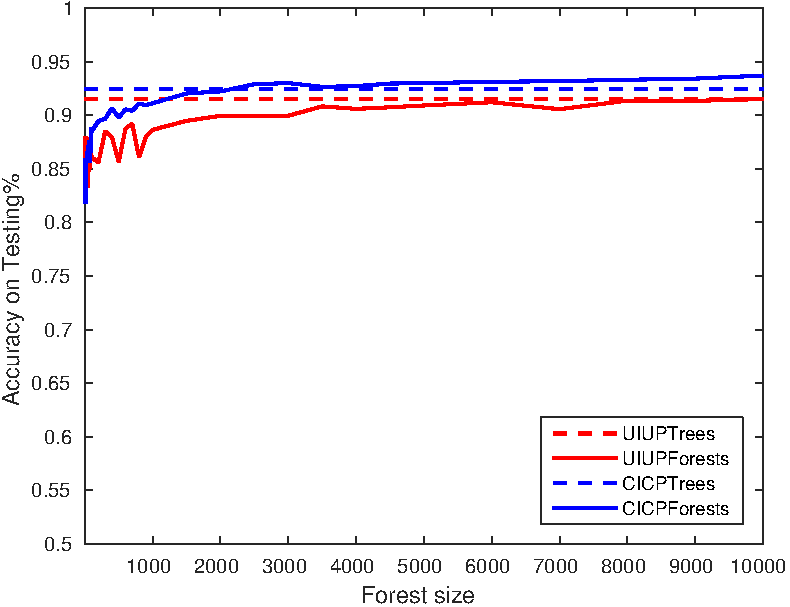
\includegraphics[width=\textwidth]{figs/PLPTF/Forests/CreditApprovalDownsampledFurther_Forests_MH.pdf}
  	\caption{CreditApproval}
		\label{fig:Crd4}
	\end{subfigure}
  \\
  \begin{subfigure}[b]{0.3\textwidth}
		\centering
  	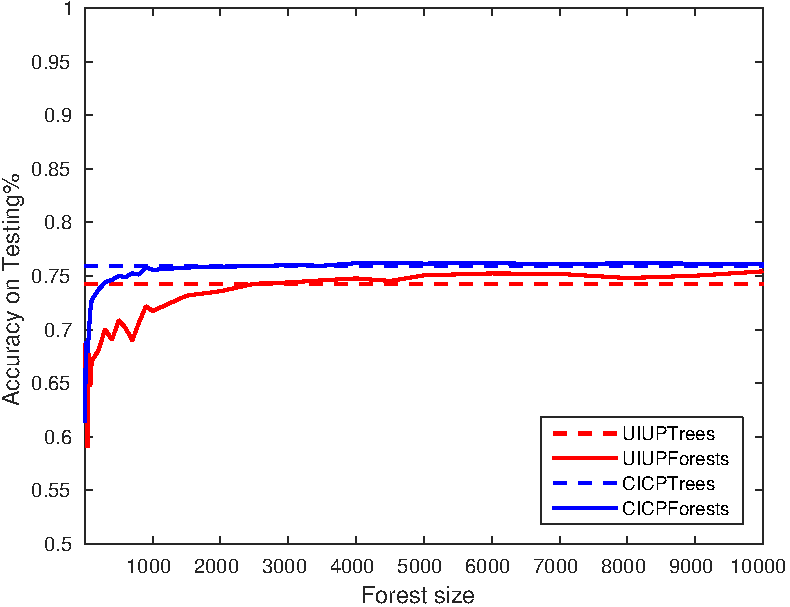
\includegraphics[width=\textwidth]{figs/PLPTF/Forests/GermanCreditDownsampledFurther_Forests_MH.pdf}
  	\caption{GermanCredit}
		\label{fig:G4}
	\end{subfigure}
  \begin{subfigure}[b]{0.3\textwidth}
		\centering
  	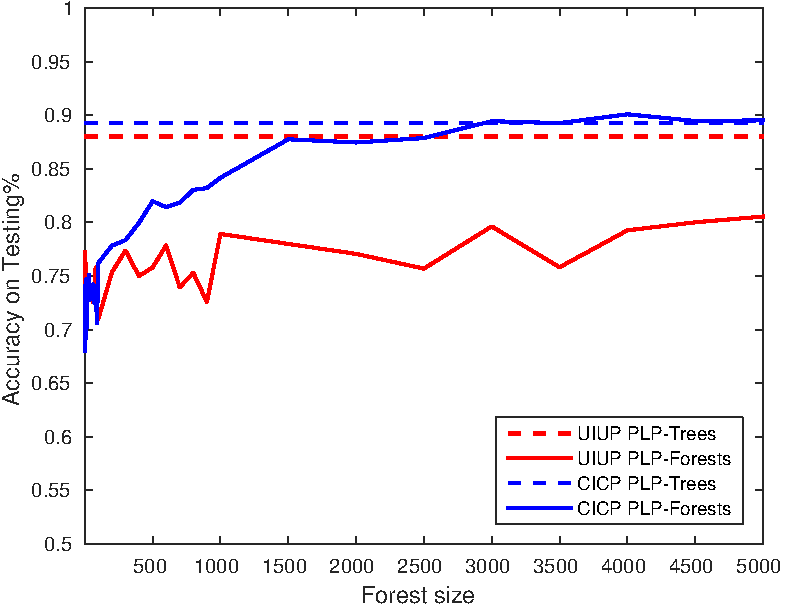
\includegraphics[width=\textwidth]{figs/PLPTF/Forests/IonosphereDownsampledFurther_Forests_MH.pdf}
  	\caption{Ionosphere}
		\label{fig:I4}
	\end{subfigure}
  \begin{subfigure}[b]{0.3\textwidth}
		\centering
  	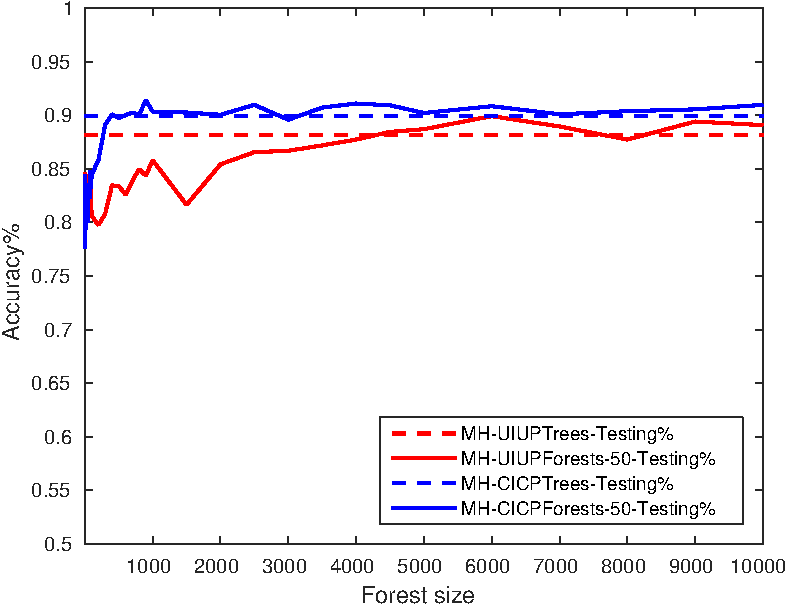
\includegraphics[width=\textwidth]{figs/PLPTF/Forests/MammographicMassDownsampled_Forests_MH.pdf}
  	\caption{MammographicMass}
		\label{fig:Mam4}
	\end{subfigure}
	\\
  \begin{subfigure}[b]{0.3\textwidth}
		\centering
  	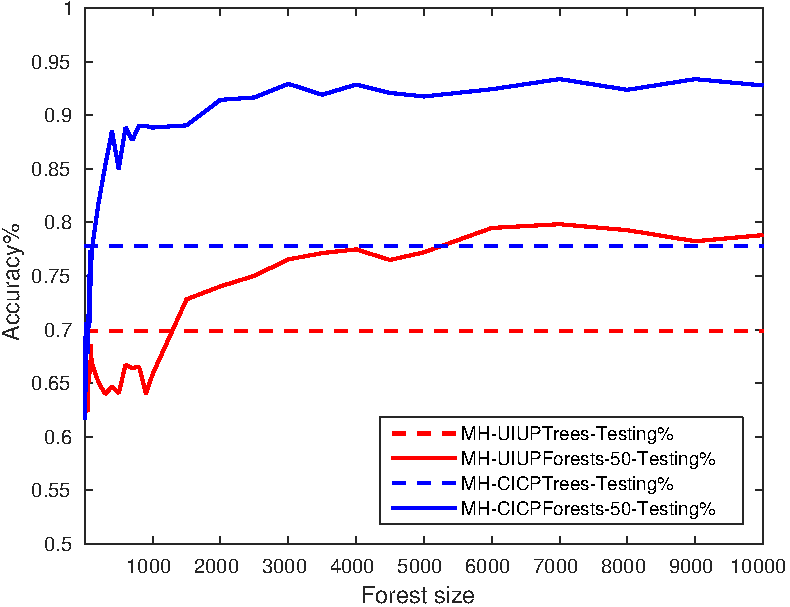
\includegraphics[width=\textwidth]{figs/PLPTF/Forests/MushroomDownsampled_Forests_MH.pdf}
  	\caption{Mushroom}
		\label{fig:Mush4}
	\end{subfigure}
  \begin{subfigure}[b]{0.3\textwidth}
		\centering
  	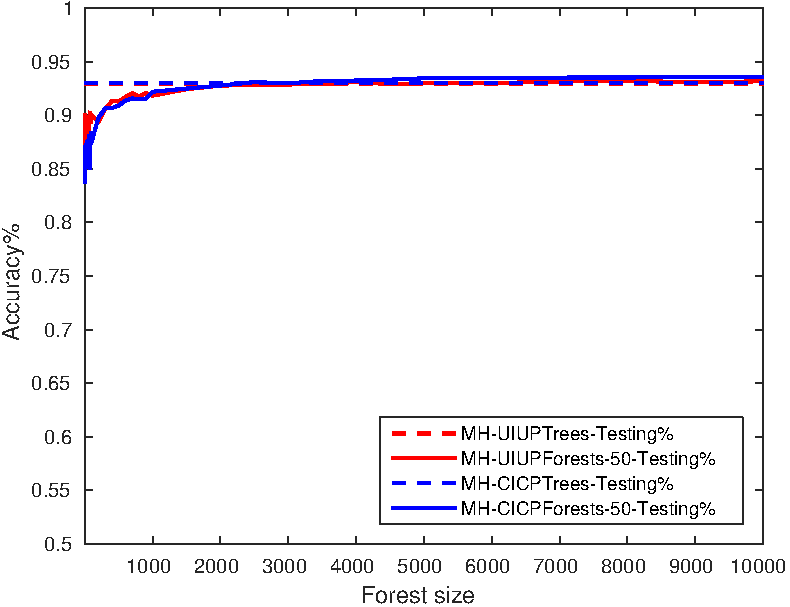
\includegraphics[width=\textwidth]{figs/PLPTF/Forests/NurseryDownsampledFurther_Forests_MH.pdf}
  	\caption{Nursery}
		\label{fig:N4}
	\end{subfigure}
  \begin{subfigure}[b]{0.3\textwidth}
		\centering
  	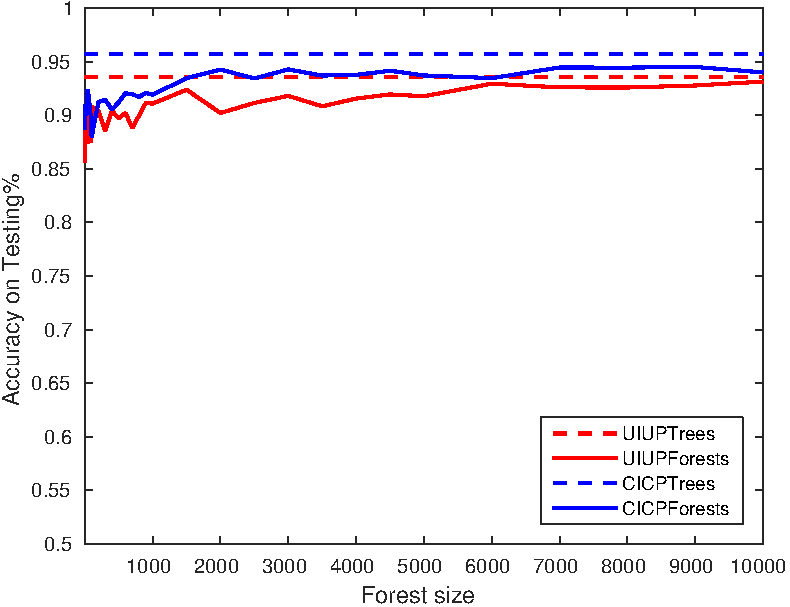
\includegraphics[width=\textwidth]{figs/PLPTF/Forests/SpectHeartDownsampledFurther_Forests_MH.pdf}
  	\caption{SPECTHeart}
		\label{fig:S4}
	\end{subfigure}
  \\
  \begin{subfigure}[b]{0.3\textwidth}
		\centering
  	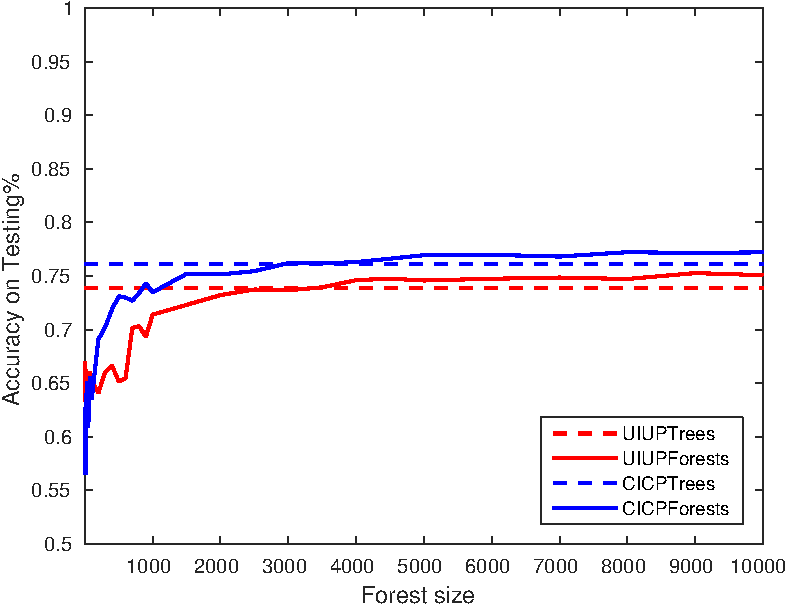
\includegraphics[width=\textwidth]{figs/PLPTF/Forests/TicTacToe_Forests_MH.pdf}
  	\caption{TicTacToe}
		\label{fig:T4}
	\end{subfigure}
  \begin{subfigure}[b]{0.3\textwidth}
		\centering
  	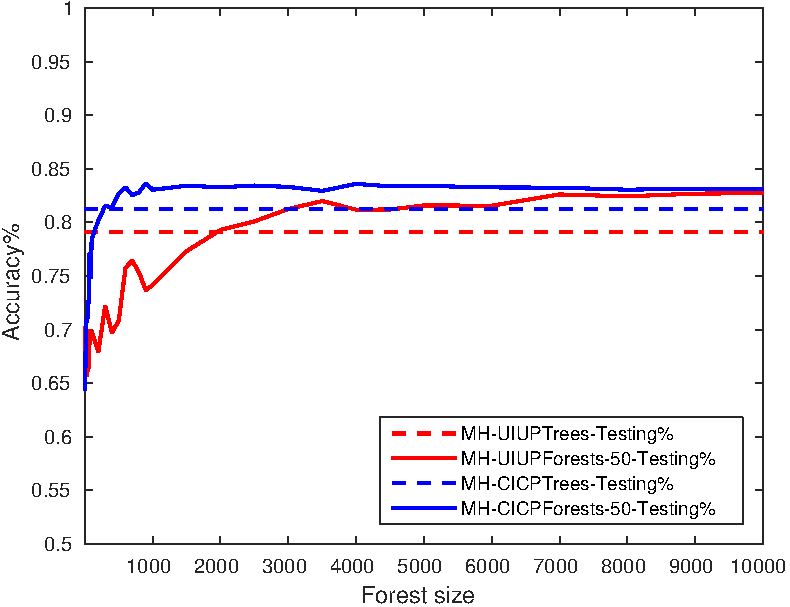
\includegraphics[width=\textwidth]{figs/PLPTF/Forests/VehicleDownsampledFurther_Forests_MH.pdf}
  	\caption{Vehicle}
		\label{fig:V4}
	\end{subfigure}
  \begin{subfigure}[b]{0.3\textwidth}
		\centering
  	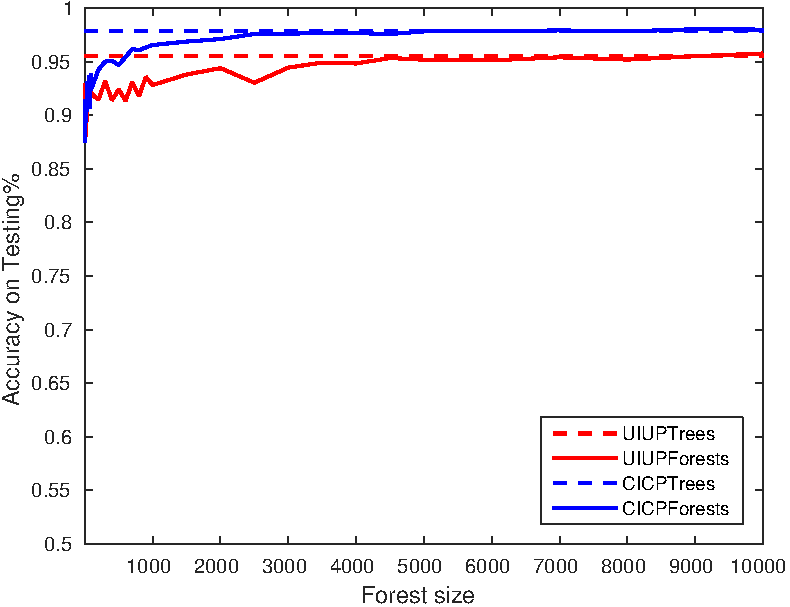
\includegraphics[width=\textwidth]{figs/PLPTF/Forests/WineDownsampled_Forests_MH.pdf}
  	\caption{Wine}
		\label{fig:W4}
	\end{subfigure}

  \caption{Forests of UIUP trees vs. forests of CICP trees}
  \label{fig:forests2}
\end{figure}

%What we have learned from \figref{forests2}:
%\begin{enumerate}
%	\item CICP forests surpass CICP trees on all but one dataset: SPECTHeart.
%	\item UIUP forests surpass CICP trees on 4 datasets, and fall short on the others.
%	\item CICP forests dominate UIUP forests on 10 datasets, and perform very close on
%				the other 2.
%\end{enumerate}

Examining \figref{forests2}, we note that with even smaller forests, consisting
of 2000 forests, the accuracies are already very close to those we observe 
for forests consisting of 5000 trees. That suggests that much larger forests
would not offer any additional boost in the accuracy.
The figure also shows that the number of trees needed in a forest in order to
offer a better accuracy than that of an individual tree varies (for only 
one case with dataset Ionosphere and class UIUP, we do not see forests 
of trees surpass individual trees in accuracy).
% mostly forests surpass or converge to trees 
%(of the same class) at some points.  One exception is UIUP PLP-forests for the
%Ionosphere dataset.
%Then, the surpass or convergence may happen when the forest is smaller or larger
%for different datasets.
%For instance, for CarEvaluation and Mushroom we need a smaller forest to beat the single tree,
%compared to a much larger forest to come close to the corresponding tree
%for Ionosphere and Wine.
%Finally, except for Ionosphere and Mushroom, we obtain results on most of the datasets that suggest 
%very comparable performances of the most restrictive class (UIUP) and 
%the most general class (CICP) across all forest sizes.

\section{Conclusions}
In this chapter, we presented results considering problems concerning learning
\tit{partial lexicographic preference trees}, or \tit{PLP-trees}.
We showed that PLP-trees are expressive preference models that can be
used to accurately model preferences arising in practical situations, and
that high-accuracy PLP-trees can be effectively computed. We also proposed
and studied a variant of the model based on the concept of a \emph{PLP-forest},
a \emph{collection} of PLP-trees, where the preference order specified by a
PLP-forest is obtained by aggregating the orders of its PLP-trees.
We proposed and implemented the best-agreement and greedy algorithms
to learn PLP-trees and PLP-forests. To support experimentation, we used
datasets that we adapted to the preference learning setting from existing
classification datasets.

Our results demonstrated the potential of both approaches. For learning 
single trees, our results show the effectiveness of the greedy heuristics 
and identify learning CIUPB trees as leading to both high accuracy and small
tree sizes. Learning PLP-forests improves accuracy and yields effective
preference models even when individual trees are learned from small example
sets. That allows us to use the best-agreement method for learning
PLP forests, the method inapplicable when example sets are large.

Looking into the future, we are interested in expanding our preference
learning library by creating real-world datasets through
conducting experiments involving human subjects.
We also plan to extend the theoretical results on the worst-case
bound for the greedy method to more general classes of PLP-trees.
Finally, we intend to implement and experiment with other aggregators
for PLP-forests, and compare with our results using
the desirable and intuitive majority rule.

